\documentclass{beamer}
% \mode<presentation>
\setbeamertemplate{navigation symbols}{}
\let\tempone\itemize
\let\temptwo\enditemize
\renewenvironment{itemize}{\tempone\addtolength{\itemsep}{0.5\baselineskip}}{\temptwo}
\usepackage{beamerthemeshadow}
\usepackage{tikz}
\usepackage{bbm}
\usepackage{multimedia}
\usepackage{hyperref}
\usepackage{natbib}
\usepackage{pgffor}
\usepackage{booktabs}
\usepackage{graphicx}
\usepackage{amssymb}
\usepackage{tabularx}
\usepackage{tikz,etoolbox}
\usepackage{tikz,amsmath,siunitx}
\usetikzlibrary{arrows,snakes,backgrounds,patterns,matrix,shapes,fit,calc,shadows,plotmarks}
\newcommand{\softmax}{\mathrm{softmax}}
\usepackage[normalem]{ulem}
\newcommand\tst{% thick strike through  %% from http://tex.stackexchange.com/questions/134088/mis-alignment-of-columns-in-tabular-environment-when-using-ulem-and-beamer
  \bgroup%
  \markoverwith{\textcolor{red}{\rule[1.1ex]{1pt}{0.8pt}}}%
  \ULon%
}

\usepackage{subcaption}
% \usepackage{url}
% \usepackage{hyperref}
\usepackage[absolute,overlay]{textpos}
\usepackage{pgf}
\usepackage{latexsym}
\usepackage{amsfonts}
\usepackage{amssymb}
\usepackage{amsthm}
\usepackage{algorithm}
\usepackage{amsmath}
\usepackage{tabularx}
\usepackage{xcolor}
\usepackage[absolute,overlay]{textpos}
\usetikzlibrary{shapes,arrows,positioning,automata,positioning,spy,matrix,scopes,chains}
\newcommand{\digs}[2]{\hphantom{999}\llap{#1}\,+\,\hphantom{999}\llap{#2}}
\setbeamersize{text margin left=6mm}
\setbeamersize{text margin right=6mm}
\renewcommand{\insertnavigation}[1]{}
\setbeamertemplate{headline}{}
\setbeamertemplate{footline}{}
\usefonttheme{professionalfonts}
\setbeamercovered{transparent}
\mode<presentation>
\linespread{1.25}
\DeclareMathOperator{\Tr}{Tr} 

\usepackage{color}
\usepackage{multirow}
\usepackage{rotating}
\usepackage[all,dvips]{xy}
\usepackage{colortbl}
\usepackage{graphicx}
\usepackage{verbatim}
\usepackage{framed}
\usepackage{natbib}
\usepackage[labelformat=empty]{caption}
\newcommand{\air}{\vspace{0.25cm}}
\newcommand{\mair}{\vspace{-0.25cm}}

\setbeamertemplate{navigation symbols}{}%remove navigation symbols
\renewcommand{\rmdefault}{crm}
\newcommand{\lnbrack}{{\normalfont [}}
\newcommand{\rnbrack}{{\normalfont ]}\thinspace}
\newcommand{\lbbrack}{\textcolor{red}{\textbf{[}}}
\newcommand{\rbbrack}{\textcolor{red}{\textbf{]}}\thinspace}
\definecolor{vermillion}{RGB}{213,94,0}
\newcommand{\given}{\,|\,}
\definecolor{orange}{RGB}{230,159,0}
\definecolor{skyblue}{RGB}{86,180,233}
\definecolor{bluegreen}{RGB}{90,143,41}
% \definecolor{bluegreen}{RGB}{0,158,115}
\definecolor{myyellow}{RGB}{240,228,66} % i dunno if this is the same as standard yellow
\definecolor{myblue}{RGB}{0,114,178}
\definecolor{vermillion}{RGB}{213,94,0}
\definecolor{redpurple}{RGB}{204,121,167}
\definecolor{lightgrey}{RGB}{234,234,234}

\newcommand{\clust}{\ensuremath{\mathrm{clust}}}
\newcommand{\loc}{\ensuremath{\mathrm{loc}}}
\newcommand{\nicein}{\ensuremath{\,{\in}\,}}
\newcommand{\niceq}{\ensuremath{\,{=}\,}}
\newcommand{\uc}{\ensuremath{\mathrm{c}}}
\newcommand{\hc}{\boldh_{\uc}}
\newcommand{\cb}{\boldb_{\mathrm{\uc}}}
\newcommand{\cW}{\boldW_{\mathrm{\uc}}}

\newcommand{\ha}{\boldh_{\ua}}
\newcommand{\hp}{\boldh_{\up}}
% \newcommand{\hc}{\boldh_{\mathrm{c}}}


\def\kargmax{\operatornamewithlimits{K-arg\,max}}
%\DeclareMathOperator{\topK}{topK}
\def\topK{\operatornamewithlimits{topK}}
\DeclareMathOperator{\suk}{succ}
\newcommand{\longpfx}[1]{\ensuremath{w_1 \cdots w_{#1}}}
\newcommand{\longgoldpfx}[1]{\ensuremath{y_1 \cdots y_{#1}}}
\newcommand{\pfx}[1]{\ensuremath{w_{1:{#1}}}}
\newcommand{\goldpfx}[1]{\ensuremath{y_{1:{#1}}}}
\newcommand{\beampred}[2]{\ensuremath{\hat{y}_{1:{#1}}^{({#2})}}}
\newcommand{\boldx}{\mathbf{x}}

\usetikzlibrary{positioning}
% \setbeamerfont{alerted text}{series=\bfseries}
% \setbeamerfont{structure}{series=\bfseries}
% Needed for diakgrams.
\def\im#1#2{
  \node(#1) [scale=#2]{\pgfbox[center,top]{\pgfuseimage{#1}}
};}
% \input{pictures_header}


\title[Seq2seq]{Interpreting, Training, and Distilling Seq2Seq Models}


\author[Alexander Rush]{Alexander Rush  (@harvardnlp) \\  
{\scriptsize  (with  Yoon Kim, Sam Wiseman, Yuntian Deng, Allen Schmaltz, Hendrik Strobelt) } \\} 

\institute[Harvard SEAS]{ \\
  \begin{center}
    
\includegraphics[width=1.3cm]{seas}
  \end{center}
  at 

  \begin{center}
    
\includegraphics[height=1.5cm]{mit}
  \end{center}
  
}
\date{}
% \usetheme{Madrid}

\newcommand{\enc}{\mathrm{src}}
\newcommand{\xvec}{\mathbf{x}}
\newcommand{\yvec}{\mathbf{y}}
\newcommand{\wvec}{\mathbf{w}}
\newcommand{\cvec}{\mathbf{c}}
\newcommand{\zvec}{\mathbf{z}}
% \newcommand{\mcY}{\mathcal{Y}}
% \newcommand{\mcV}{\mathcal{V}}
\newcommand{\context}{\mathbf{w}_{\mathrm{c}}}
\newcommand{\embcontext}{\mathbf{\tilde{w}}_{\mathrm{c}}}
\newcommand{\inpcontext}{\mathbf{\tilde{x}}}
\newcommand{\start}{\mathbf{\tilde{y}}_{\mathrm{c0}}}
\newcommand{\End}{\mathrm{\texttt{</s>}}}

\newcommand{\Uvec}{\mathbf{U}}
\newcommand{\Evec}{\mathbf{E}}
\newcommand{\Gvec}{\mathbf{G}}
\newcommand{\Fvec}{\mathbf{F}}
\newcommand{\Pvec}{\mathbf{P}}
\newcommand{\pvec}{\mathbf{p}}
\newcommand{\Qvec}{\mathbf{Q}}
\newcommand{\Vvec}{\mathbf{V}}
\newcommand{\Wvec}{\mathbf{W}}
\newcommand{\hvec}{\mathbf{h}}
% \newcommand{\reals}{\mathbb{R}}

\newcommand{\Cite}[1]{{\footnotesize \citep{#1}}}
\newcommand{\TT}[1]{{\footnotesize\tt{#1}}}
\newcommand{\boldw}{\boldsymbol{w}}
\newcommand{\boldu}{\boldsymbol{u}}
\newcommand{\boldv}{\boldsymbol{v}}
\newcommand{\boldb}{\boldsymbol{b}}
\newcommand{\boldW}{\boldsymbol{W}}
\newcommand{\boldh}{\boldsymbol{h}}
\newcommand{\boldg}{\boldsymbol{g}}
\newcommand{\ua}{\ensuremath{\mathrm{a}}}
\newcommand{\up}{\ensuremath{\mathrm{p}}}
%\newcommand{\bphi}{\ensuremath{\mathbf{\phi}}}
\newcommand{\bphi}{\boldsymbol{\phi}}
\newcommand{\btheta}{\boldsymbol{\theta}}
\newcommand{\mcY}{\mathcal{Y}}
\newcommand{\mcX}{\mathcal{X}}
\newcommand{\mcC}{\mathcal{C}}
\newcommand{\mcA}{\mathcal{A}}
\newcommand{\mcV}{\mathcal{V}}
\newcommand{\trans}{\ensuremath{\mathsf{T}}}
\def\argmin{\operatornamewithlimits{arg\,min}}
\def\argmax{\operatornamewithlimits{arg\,max}}
\newcommand{\reals}{\ensuremath{\mathbb{R}}}

\newcommand{\aphi}{\boldsymbol{\phi}_{\mathrm{a}}}
\newcommand{\pwphi}{\boldsymbol{\phi}_{\mathrm{p}}}
\newcommand{\squigaphi}{\widetilde{\boldsymbol{\phi}}_{\mathrm{a}}}
\newcommand{\squigpwphi}{\widetilde{\boldsymbol{\phi}}_{\mathrm{p}}}

\newcommand{\aW}{\boldW_{\mathrm{\ua}}}
\newcommand{\pW}{\boldW_{\mathrm{\up}}}

\newcommand{\ab}{\boldb_{\mathrm{\ua}}}
\newcommand{\pb}{\boldb_{\mathrm{\up}}}

\newcommand{\Da}{d_{\mathrm{a}}}
\newcommand{\Dp}{d_{\mathrm{p}}}

% \newcommand{\ha}{\boldh_{\ua}}
% \newcommand{\hp}{\boldh_{\up}}

\newcommand{\ourmodel}{This work}
\newcommand{\zro}{{\color{white}0}}


\def\argmax{\operatornamewithlimits{arg\,max}}
\def\kargmax{\operatornamewithlimits{K-arg\,max}}

\begin{document}

\begin{frame}
  \titlepage
\end{frame}

% \begin{frame}
%   \begin{block}{}
%     \begin{quote}
%       Although current deep learning research tends to claim to
%       encompass NLP, I'm (1) much less convinced about the strength of
%       the results, compared to the results in, say, vision ...
%     \end{quote}
%   \end{block}
%   \begin{flushright}
%     - Michael Jordan (2014) (quoted in Chris Manning, ``Computational Linguistics and Deep Learning'')
%   \end{flushright}
% \end{frame}

\begin{frame}
  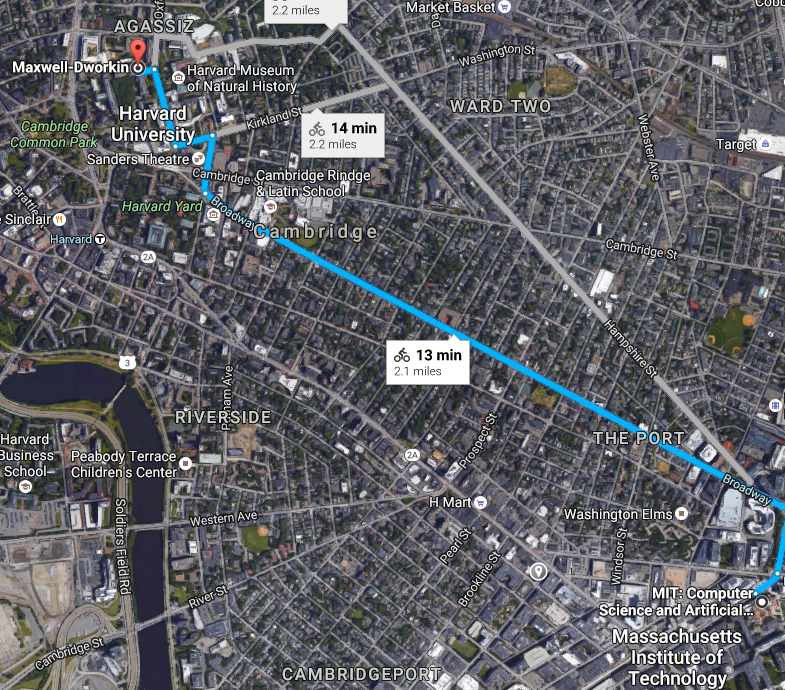
\includegraphics[width=1\textwidth]{harvardmap}
\end{frame}

\begin{frame}{}
  \begin{center}
    \structure{Sequence-to-Sequence}
  \end{center}

  \begin{itemize}
  \item \alert<2>{Machine Translation} \Cite{kalchbrenner2013recurrent,sutskever2014sequence, Cho2014, bahdanau2014neural,luong15effective} 
    \air

   
  \item Question Answering \Cite{Hermann2015} 
  \item Conversation \Cite{Vinyals2015} \Cite{Serban2016}
  \item Parsing \Cite{vinyals15grammar}
  \item Speech \Cite{Chorowski2015,Chan2015}
  \item Caption Generation \Cite{karpathy2015deep,Xu2015,Vinyals2015b}
  \item Video-Generation \Cite{Srivastava2015a}
  \item NER/POS-Tagging \Cite{Gillick2016}
  \item Summarization \Cite{Rush2015} 
    \air 

  \end{itemize}
  
\end{frame}


\begin{frame}{}
  \begin{center}
    What's ML aspects have defined NLP problems? 
  \end{center}

  \begin{enumerate}
    \air
  \item  Large, discrete input state spaces.
    \begin{itemize}
    \item Vocabulary sizes in $10,000 - 100,000$
    \end{itemize}
    \air
  \item  Long-term dependencies
    \begin{itemize}
    \item \textit{Sasha is  giving a talk today at MIT, $\ldots$, he is excited}.  
    \end{itemize}
    \air
  \item Variable-length output spaces 
    \begin{itemize}
    \item  e.g. sentences, documents, conversations
    \end{itemize}
    \air
  \end{enumerate}
\end{frame}


\begin{frame}
  \begin{center}
    \alert{Seq2Seq Neural Network Toolbox}
    \air 
  \end{center}
  \begin{center}
    \begin{tabular}{cclll}
      \structure{Embeddings} & & sparse features &$\Rightarrow$& dense features \\\\
      \structure{RNNs} & & feature sequences & $\Rightarrow$ &dense features \\\\
      \structure{Softmax} & & dense features & $\Rightarrow$ & discrete predictions \\
    \end{tabular}
  \end{center}
\end{frame}

\begin{frame}
  \begin{center}
    \begin{tabular}{cclll}
      \structure{Embeddings} & & sparse features & $\Rightarrow$ & dense features \\\\
    \end{tabular}
  \end{center}

  \begin{center}
    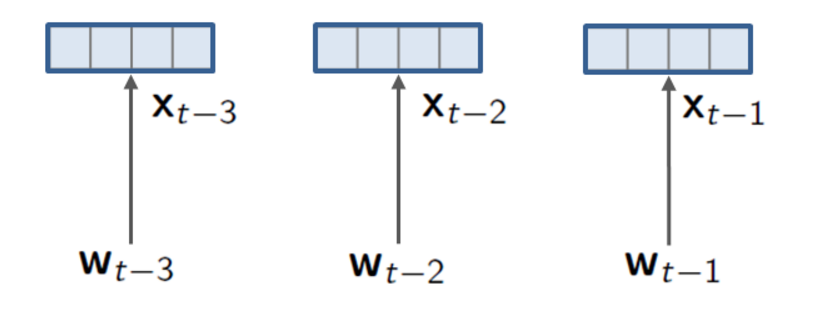
\includegraphics[width=7cm]{emb}
  \end{center}
\end{frame}

\begin{frame}
  \begin{center}
    \includegraphics[height=0.9\textheight]{graph}

    \href[pdfnewwindow=true]{http://harvardnlp.github.io/seq2seq-talk/web/wordvecs.html}{[Words Vectors]}
   \end{center}
\end{frame}


\begin{frame}
  \begin{center}
    \begin{tabular}{cclll}
      \structure{RNNs/LSTMs} & & feature sequences & $\Rightarrow$ &dense features \\\\
    \end{tabular}
  \end{center}


  \begin{center}
    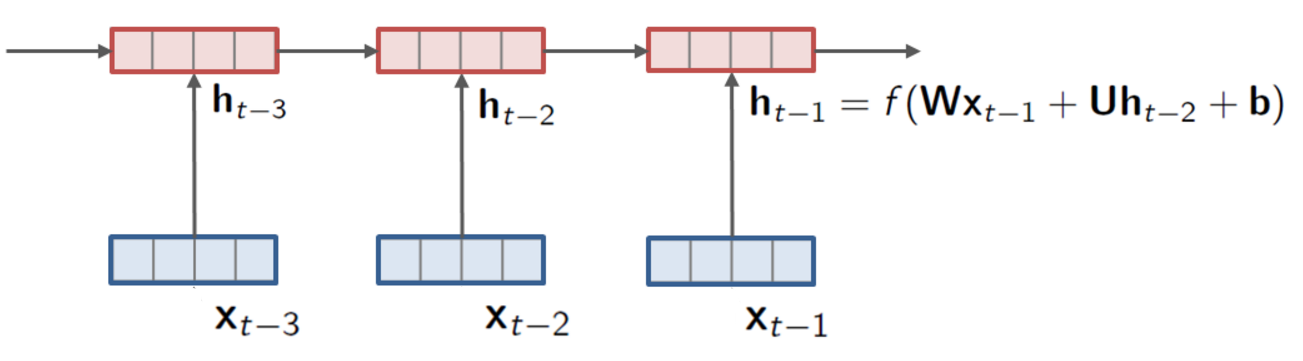
\includegraphics[width=11cm]{rnn}
  \end{center}  
\end{frame}



\begin{frame}
  \begin{center}
    \begin{tabular}{cclll}
      \structure{LM/Softmax} & & dense features & $\Rightarrow$ & discrete predictions \\
    \end{tabular}
    \air 

    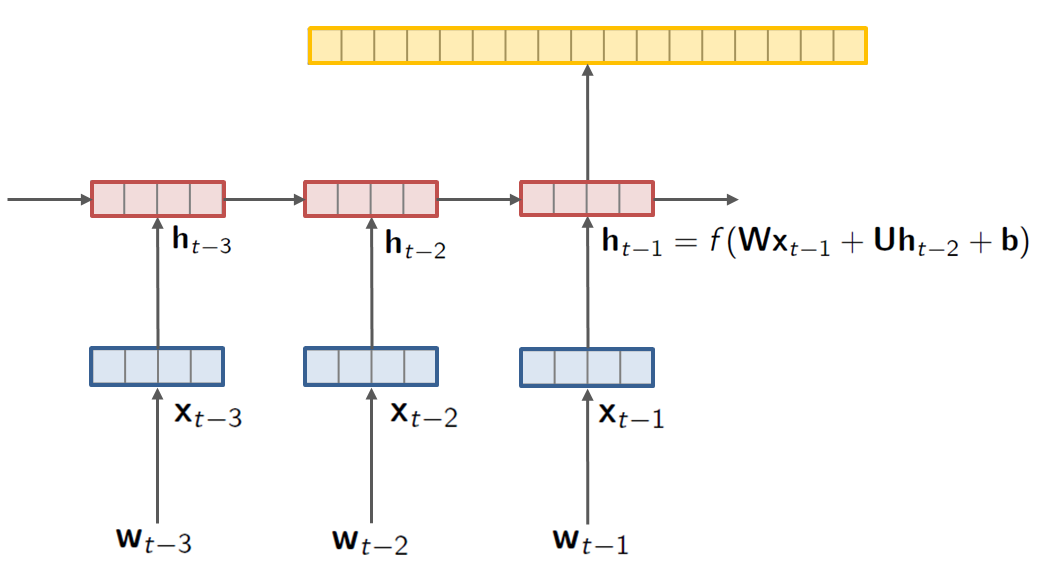
\includegraphics[width=0.8\textwidth]{rnnlm5}
  \end{center}
  \[ p(w_t | w_1, \ldots, w_{t-1}; \theta) = \text{softmax}(\mathbf{W}_{out} \mathbf{h}_{t-1} + \mathbf{b}_{out}) \] 

  \[ p(w_{1:T} ) = \prod_{t} p(w_t | w_1, \ldots, w_{t-1}) \] 
    % \caption{Xu et al (2015)}  
\end{frame}

\begin{frame}
  \begin{center}
    \structure{Contextual Language Model / ``seq2seq''}
  \end{center}
    \air 
   
    \begin{center}
      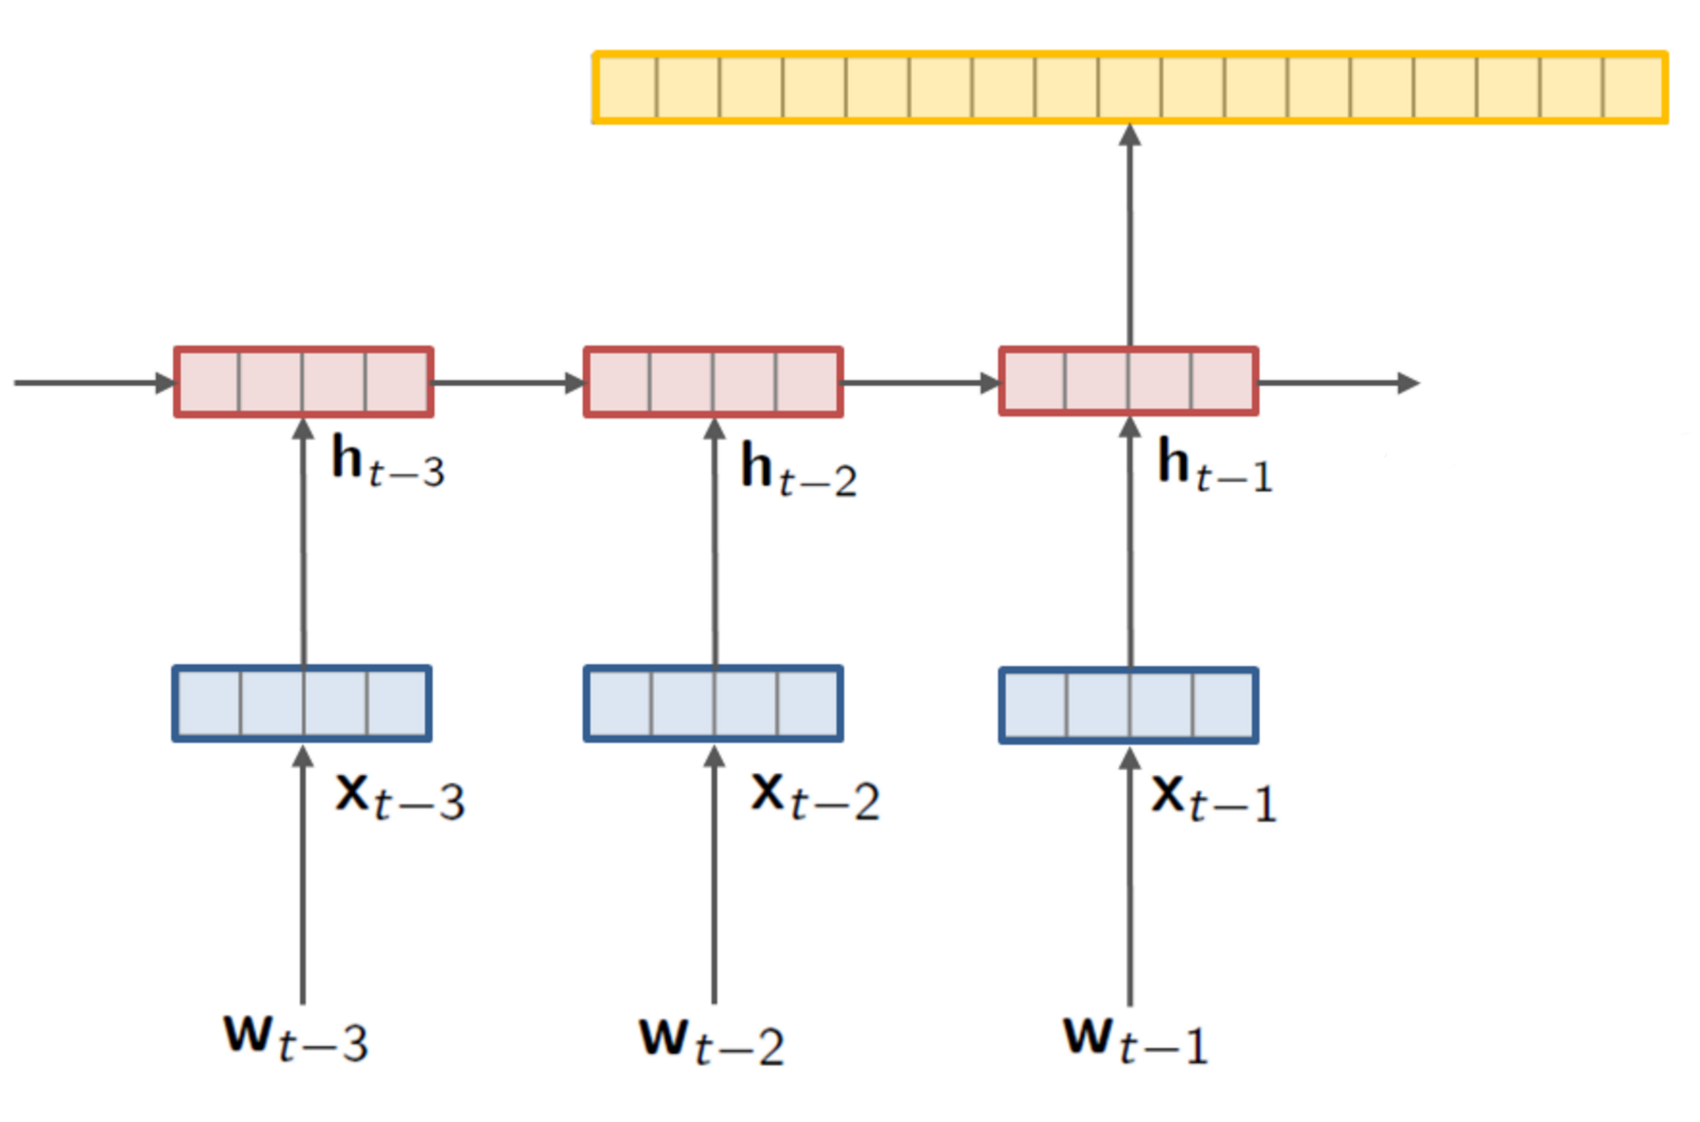
\includegraphics[width=0.6\textwidth]{rnnlm6}
    \end{center}
  \begin{itemize}
  \item Key idea, contextual language model based on encoder $\cvec$: 
  \end{itemize}
  \[ p(w_{1:T} | \cvec) = \prod_{t} p(w_t | w_1, \ldots, w_{t-1}, \cvec) \] 
  
\end{frame}


\begin{frame}
  \begin{center}
    Actual Seq2Seq / Encoder-Decoder / Attention-Based Models
  \end{center}
    \begin{center}
      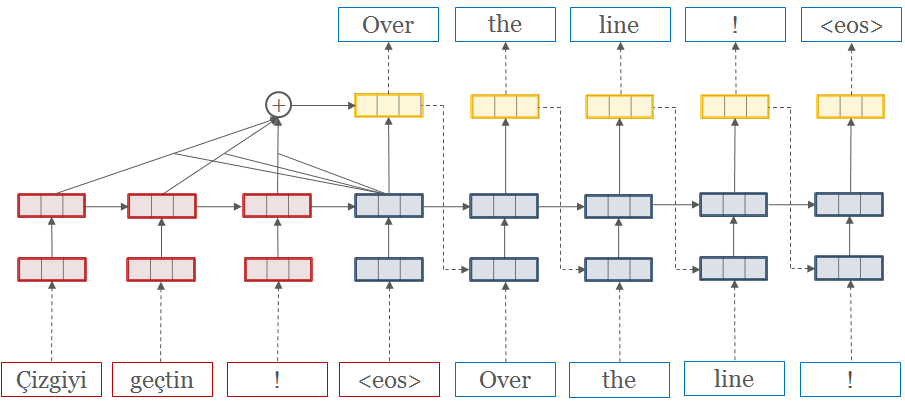
\includegraphics[width=0.7\textwidth]{simple-attn}
    \end{center}
  \begin{itemize}
  \item Different encoders, attention mechanisms, input feeding, ...
    \air
  \item Almost all models use LSTMs or other gated RNNs 
    \air
  \item Large multi-layer networks  necessary for good performance.
    \begin{itemize}
    \item 4 layer, 1000 hidden dims is common for MT
    \end{itemize}
  % \item Main idea, contextual language model based on encoder $\cvec$: 
  \end{itemize}
  % \[ p(w_{1:T} | \cvec) = \prod_{t} p(w_t | w_1, \ldots, w_{t-1}, \cvec) \] 
\end{frame}


\begin{frame}
  \centerline{\textbf{Seq2Seq-Attn}   }

  \begin{itemize}
  \item HarvardNLP's open-source system (Yoon Kim) \href[pdfnewwindow=true]{http://github.com/harvardnlp/seq2seq-attn}{http://github.com/harvardnlp/seq2seq-attn}
    \air 
  \item Used by SYSTRAN for 32 language pairs \Cite{systran}
  \end{itemize}
  
  \begin{center}
    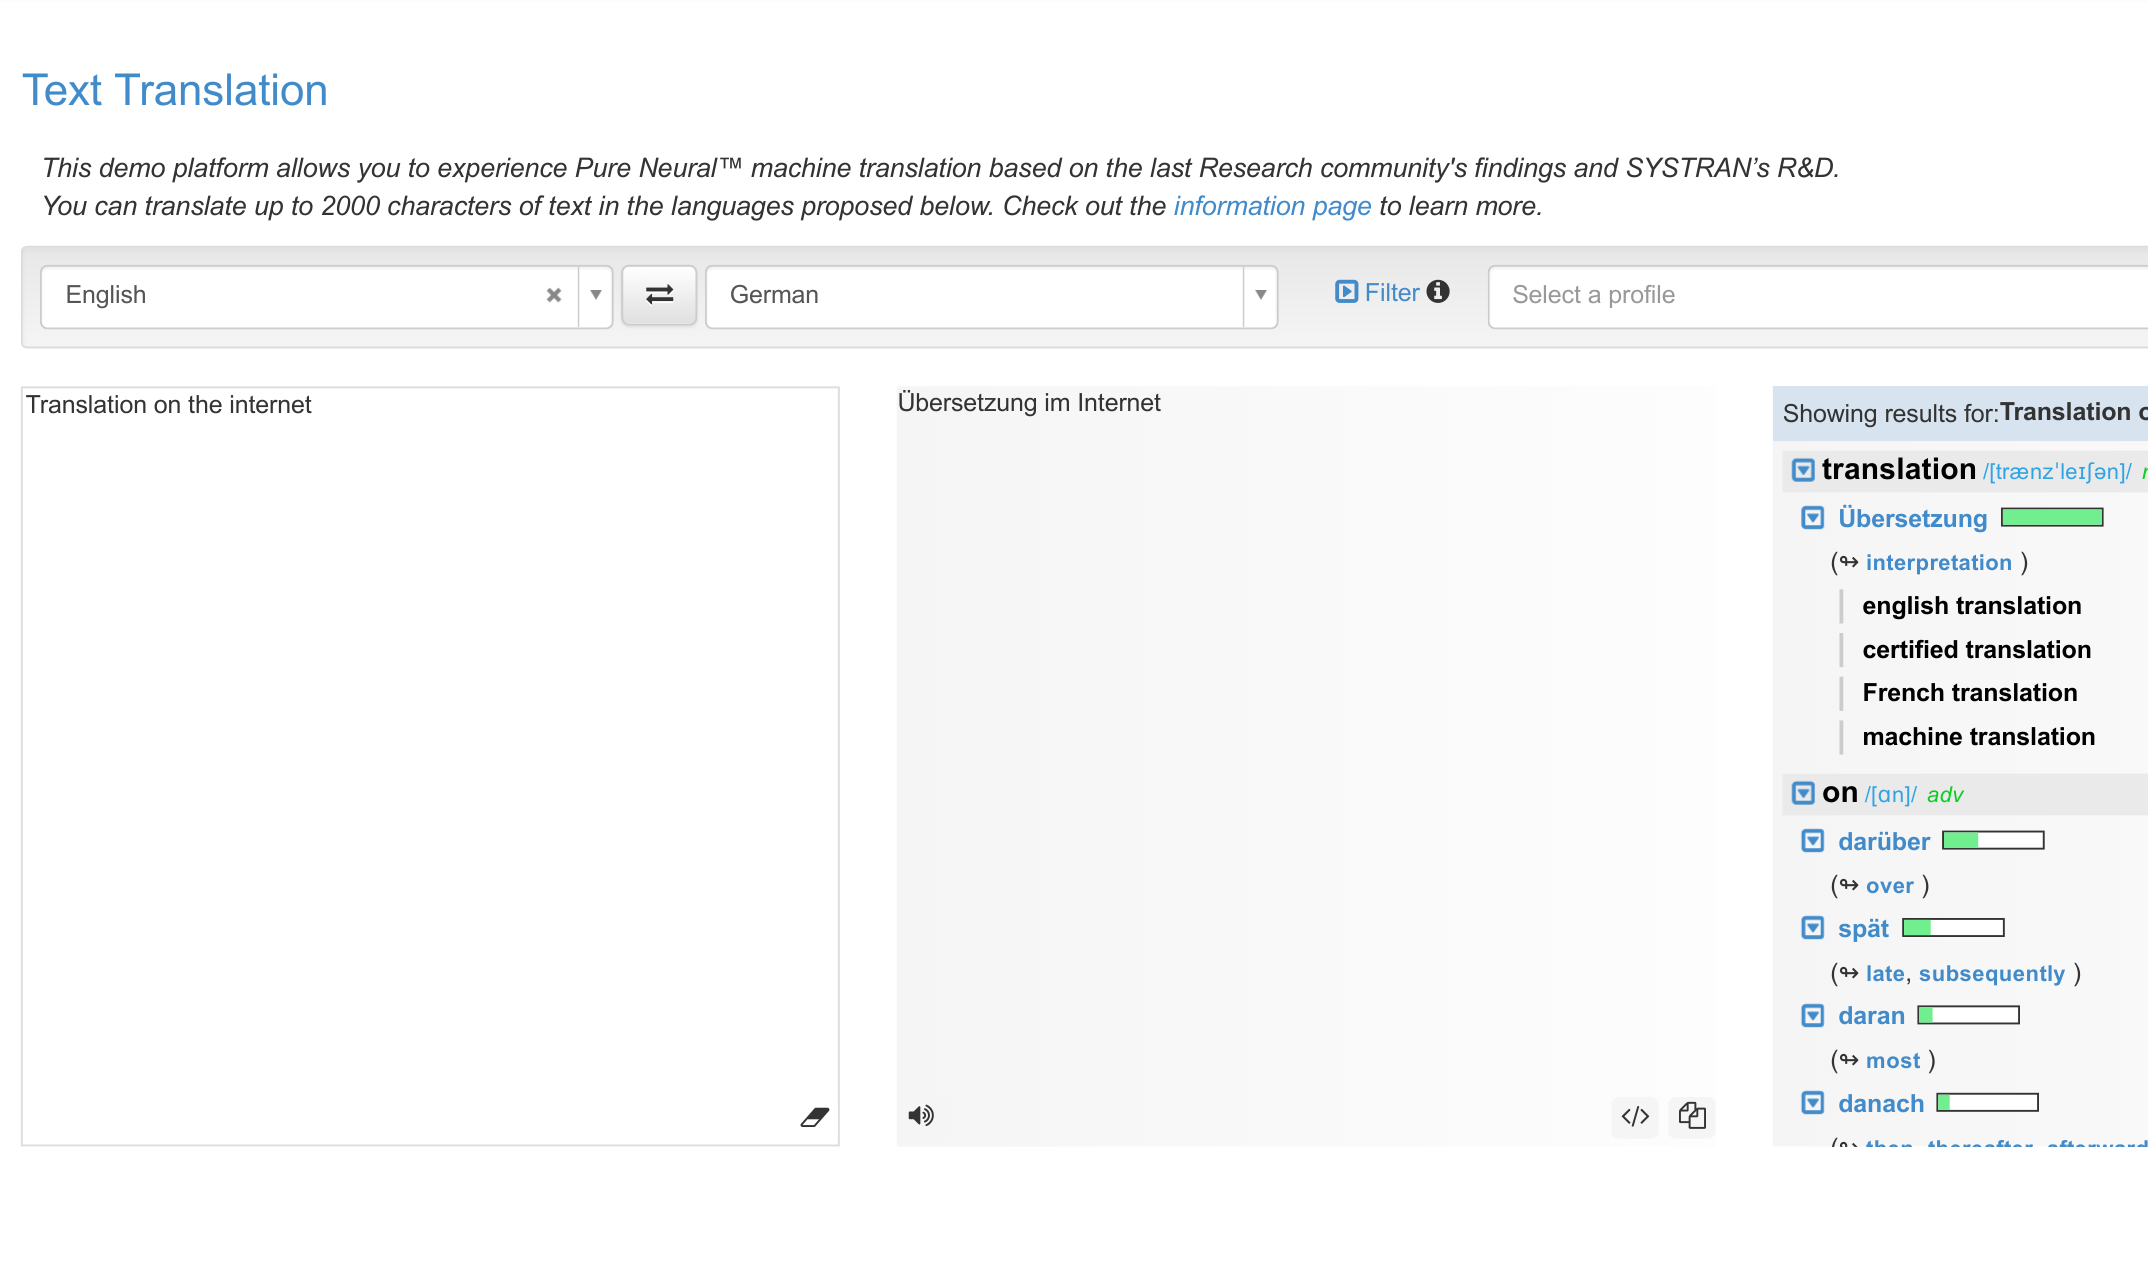
\includegraphics[width=0.9\textwidth]{systran}

    \href[pdfnewwindow=true]{http://demo-pnmt.systran.net}{[Demo]}
  \end{center}

\end{frame}


\begin{frame}
  \centerline{\textbf{Seq2Seq Applications:} \alert{Neural Summarization} \Cite{Rush2015} }
  \begin{center}
    \textbf{Source} (First Sentence)
  \end{center}
  
  \begin{figure}
    \textit{\structure<2>{Russian Defense Minister Ivanov}
      called \structure<2>{Sunday} for the creation of
      a joint front \structure<2>{for combating} global terrorism. }
  \end{figure}

  \begin{center}
    \textbf{Target} (Title)
  \end{center}
  \mair

  \begin{figure}
    \centering
    \textit{\alert<2>{Russia} calls for joint
      front \alert<2>{against} terrorism.}
  \end{figure}

\air
\air

  \begin{itemize}
  \item \Cite{mou2015backward} \Cite{cheng2016neural} \Cite{toutanovadataset} \Cite{wang2016experimental} \Cite{takaseneural}, among others
  \item Used by Washington Post to suggest headlines \Cite{shuguangwang}
  \end{itemize}
\end{frame}

\begin{frame}
  \centerline{\textbf{Seq2Seq Applications:} \alert{Grammar Correction} \Cite{Schmaltz2016} }
  % \centerline{\structure{Grammar Correction} \cite{}}
  
  \begin{center}
    \textbf{Source} (Original Sentence)
  \end{center}
  
  \begin{figure}
    \textit{There is no \structure{a doubt}, tracking \structure{systems has} brought many benefits in this information
age . }
  \end{figure}

  \begin{center}
    \textbf{Target} (Corrected Sentence)
  \end{center}
  \mair

  \begin{figure}
    \centering
    \textit{There is no doubt, tracking systems have
      brought many benefits in this information
      age . }
  \end{figure}

  \begin{itemize}
  \item 1st on BEA'11 grammar correction task \Cite{Daudaravicius2016}
  \end{itemize}
\end{frame}


\begin{frame}
  \centerline{\textbf{Seq2Seq Applications:} \alert{Im2Markup} (Deng and Rush, 2016) }
  
  \air 

  \begin{center}
    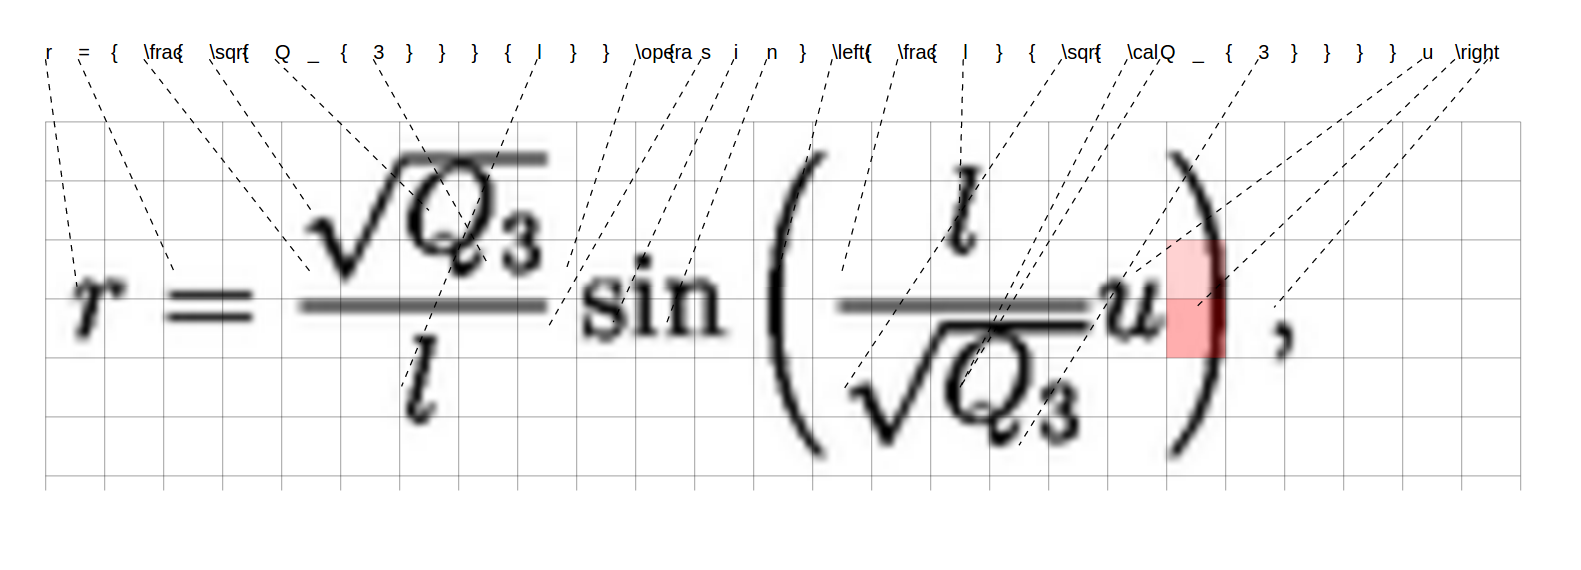
\includegraphics[width=\textwidth]{math}
  \end{center}
  % \movie[width=\textwidth, height=4cm, poster, repeat]{}{Latex.mp4}
  


  \begin{figure}
    \centering
  \end{figure}

  \centerline{\href[pdfnewwindow=true]{https://harvardnlp.github.io/seq2seq-talk/web/math.html}{[Latex Example]}}
  \centerline{\href[pdfnewwindow=true]{https://lstm.seas.harvard.edu/latex}{[Project]}}
\end{frame}


\begin{frame}
  \centerline{\structure{This Talk}}
  \air 
  \air

  \begin{itemize}
  \item How can we \textbf{interpret} these learned hidden representations? 
    \air 

    

  \item  How should we \textbf{train} these style of models? 
    \air 
  \item  How can we \textbf{shrink} these models for practical applications? 
  \end{itemize}
\end{frame}


\begin{frame}
  \centerline{\structure{This Talk}}
  \air 
  \air

  \begin{itemize}
  \item How can we \textbf{interpret} these learned hidden representations? 

    \begin{center}
      \alert{LSTMVis}   
      \href[pdfnewwindow=true]{https://lstm.seas.harvard.edu/}{lstm.seas.harvard.edu}

      \Cite{Strobelt2016}

      
\includegraphics[width=2cm]{hen}
    \end{center}


    \air 

    

  \item  \textcolor{gray}{How should we \textbf{train} these style of models? \Cite{Wiseman2016a}}
    \air 
  \item  \textcolor{gray}{How can we \textbf{shrink} these models for practical applications? \Cite{Kim2016a}}
  \end{itemize}
\end{frame}

\section{Interpretation}

% \begin{frame}
%   \air 
%   \includegraphics[width=\textwidth,trim={0 0 0 19.5cm},clip]{filters}
%   \begin{center}
%      \Cite{DBLP:conf/eccv/ZeilerF14}
%   \end{center}
% \end{frame}

% \begin{frame}
%   \begin{frame}
%   \begin{center}
%     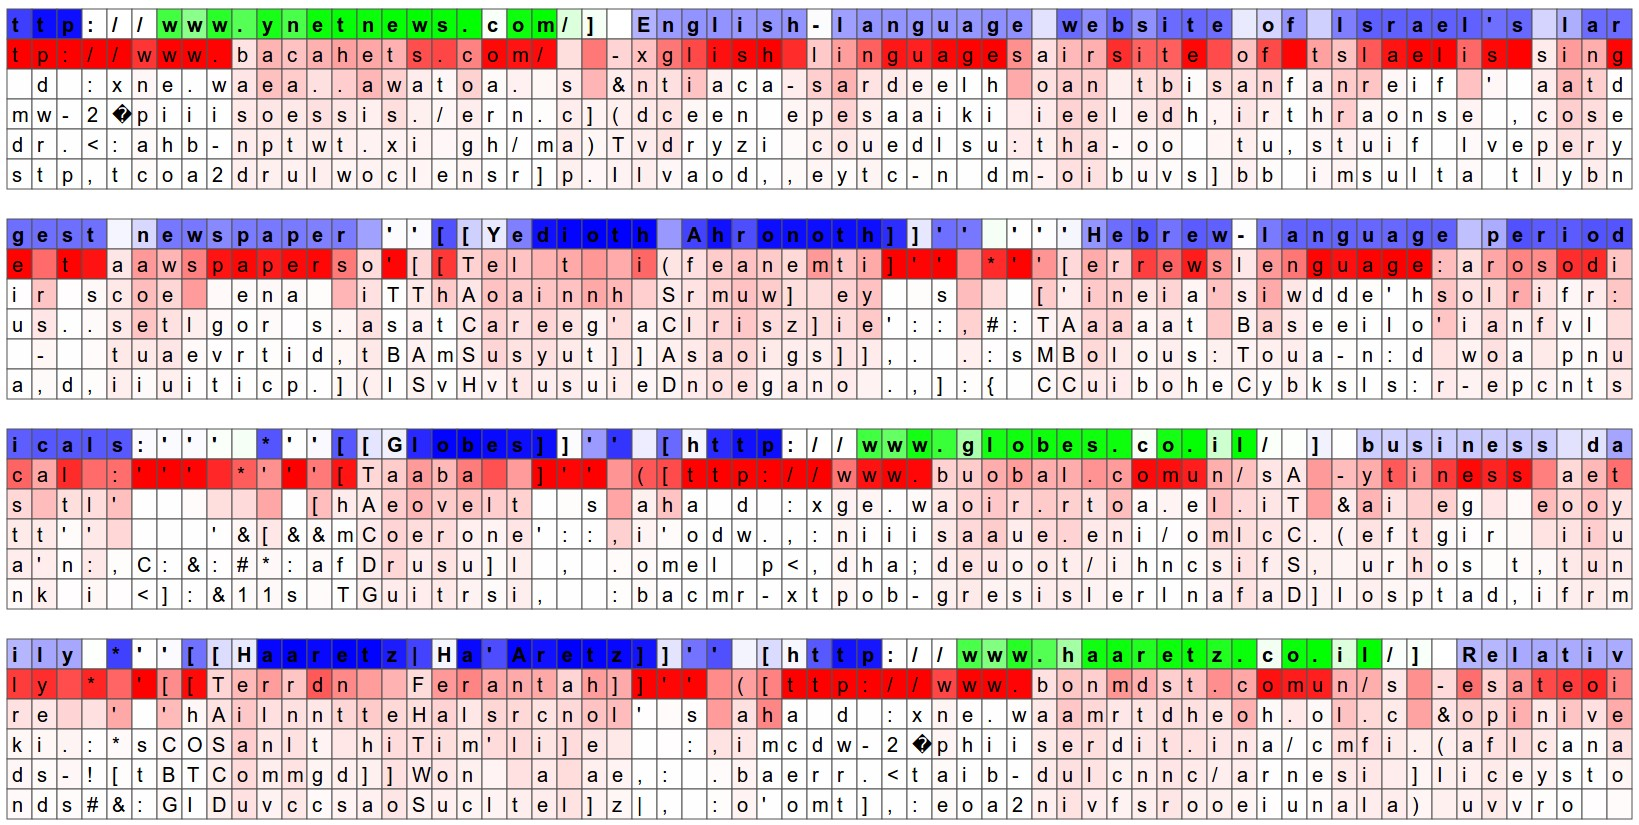
\includegraphics[width=\textwidth]{lstm1}

%     {\footnotesize (Karpathy et al, 2015)}
%   \end{center}

%     % \caption{Xu et al (2015)}  
% \end{frame}


\begin{frame}
  % \begin{frame}
  \centerline{Vector-Space RNN Representation}
  \begin{center}
    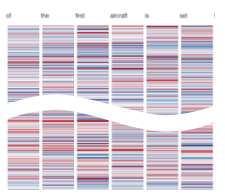
\includegraphics[height=5cm]{lstmrep}
  \begin{center}
    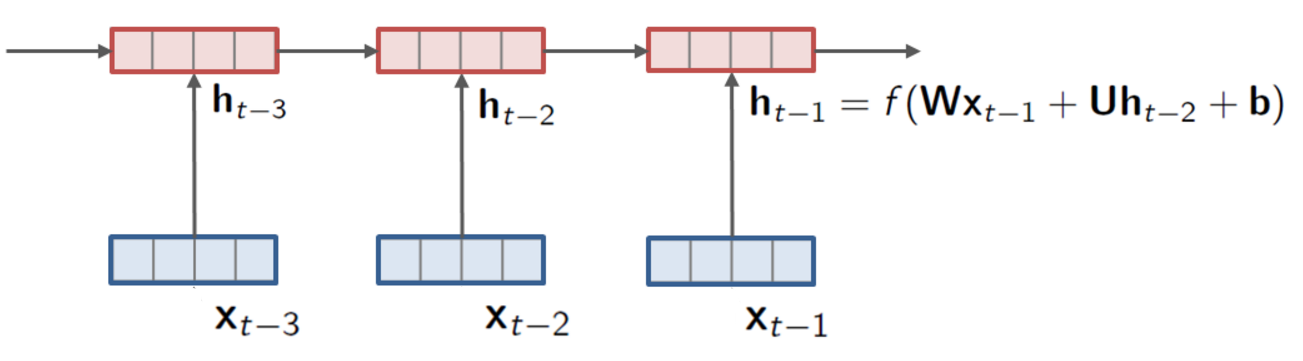
\includegraphics[width=11cm]{rnn}
  \end{center}
  \end{center}
\end{frame}


\begin{frame}
  % \begin{frame}
  \begin{center}
    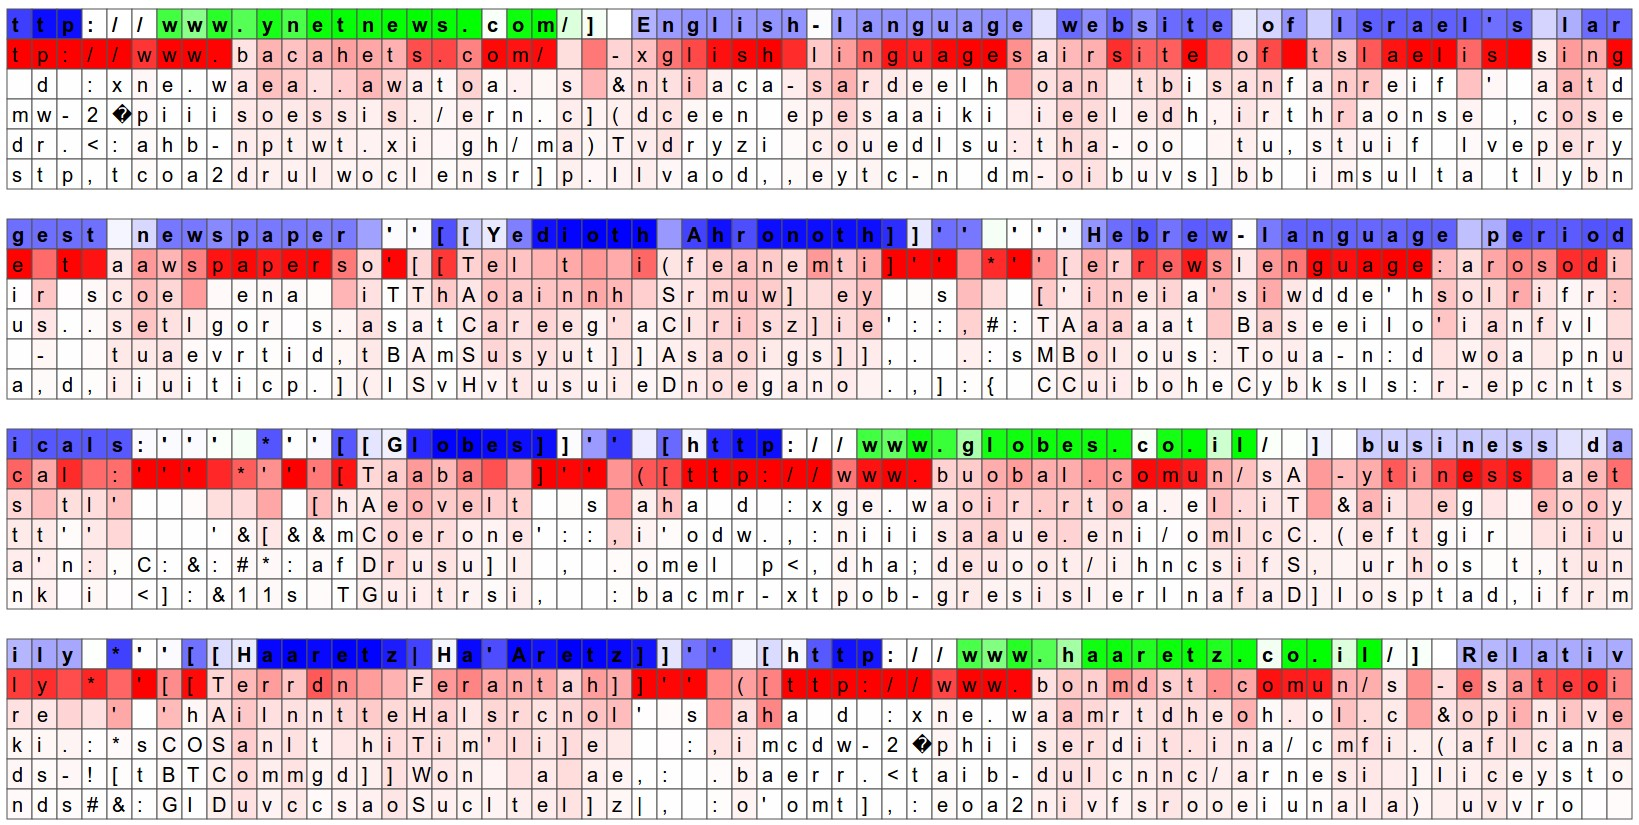
\includegraphics[width=\textwidth]{lstm1}

     \Cite{karpathy2015visualizing}
    % {\footnotesize (Karpathy et al, 2015)}
  \end{center}
    % \caption{Xu et al (2015)}  
\end{frame}

\begin{frame}
  \centerline{\alert{Example 1}: Synthetic (Finite-State) Language}
  \air

  \begin{center}
    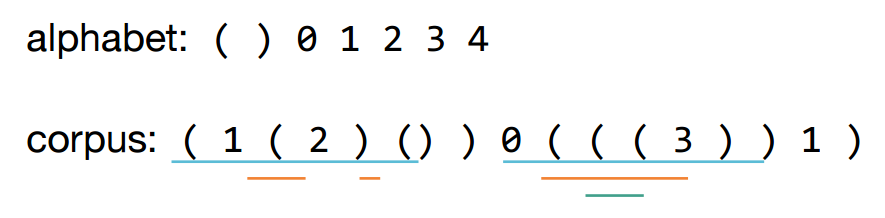
\includegraphics[width=9cm]{parenlang}
  \end{center}
  \mair

  \begin{itemize}
  \item Numbers are randomly generated, must match nesting level.
    \air

  \item Train a predict-next-word language model (decoder-only).
  \end{itemize}
    \[ p(w_t | w_1, \ldots, w_{t-1}) \] 
  
\air
  \centerline{\href[pdfnewwindow=true]{http://lstm.seas.harvard.edu/client/pattern_finder.html?data_set=00parens&source=states::states2&pos=150}{[Parens Example]}}
\end{frame}


\begin{frame}
  \centerline{\alert{Example 2}: Real Language}
  \air

  \begin{description}
  \item[alphabet:] all english words
  \item[corpus:] Project Gutenberg Children's books 
  \end{description}
  % \begin{center}
  %   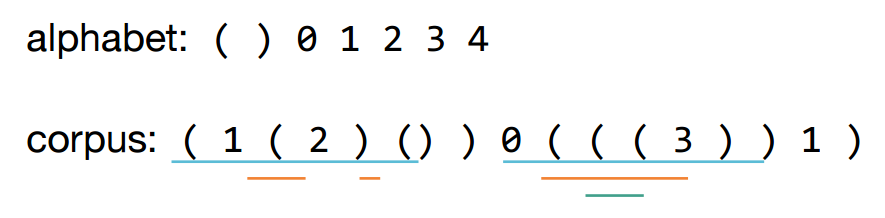
\includegraphics[width=9cm]{parenlang}
  % \end{center}

  \begin{itemize}
  % \item 
  %   \air

  \item Train a predict-next-word language model (decoder-only).

  
  \end{itemize}
    \[ p(w_t | w_1, \ldots, w_{t-1}) \] 

\air
  \centerline{ \href[pdfnewwindow=true]{http://lstm.seas.harvard.edu/client/pattern_finder.html?data_set=05childbook&source=states::states1&pos=100}{[LM Example]}}
\end{frame}


\begin{frame}
  \centerline{\alert{Example 3}: Seq2Seq Encoder}
  \air

  \begin{description}
  \item[alphabet:] all english words
  \item[corpus:]  Summarization
  \end{description}
  % \begin{center}
  %   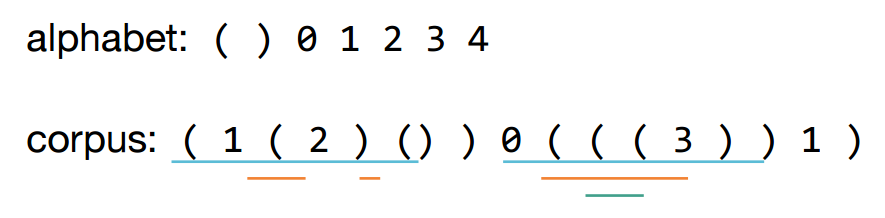
\includegraphics[width=9cm]{parenlang}
  % \end{center}

  \begin{itemize}
  % \item 
  %   \air

  \item Train a full seq2seq model, examine \textit{encoder} LSTM.
  
  \end{itemize}


\air
  \centerline{ \href[pdfnewwindow=true]{http://lstm.seas.harvard.edu/client/pattern_finder.html?data_set=20autoencoder&source=states::states2&pos=100}{[Summarization Example]}}
\end{frame}
\begin{frame}
  \centerline{\structure{This Talk}}
  \air 
  \air

  \begin{itemize}
  \item \textcolor{gray}{How can we \textbf{interpret} these learned hidden representations? \Cite{Strobelt2016}}
    \air 
  \item  How should we \textbf{train} these style of models? 
    \air 

    \begin{center}
      \alert{Sequence-to-Sequence Learning as Beam-Search
        Optimization}
     
      \Cite{Wiseman2016a}

      
\includegraphics[width=2cm]{sam}
    \end{center}


    \air 
  \item \textcolor{gray}{ How can we \textbf{shrink} these models for practical applications \Cite{Kim2016a}? }
  \end{itemize}
\end{frame}

\begin{frame}
  \centerline{Seq2Seq Notation}
 
  \begin{itemize}
  \item $x$; source input 
  \item $\cal V$; vocabulary
  \item $w_t$; random variable for the $t$-th target token with support $\mcV$ 
  \item $y_{1:T}$; ground-truth output 
  \item $\hat{y}_{1:T}$; predicted output 
  \item  $p(w_{1:T} \given x ;\theta)= \prod_{t} p(w_t | w_{1:t-1}, x; \theta)$; model distribution \
  \end{itemize}
\end{frame}


\begin{frame}
  \textbf{\structure{Train Objective}}: Given source-target pairs $(x, y_{1:T})$, minimize NLL of each word independently, conditioned on \textit{gold} history $y_{1:t-1}$
\begin{align*}
{\cal L}_{\text{NLL}}(\theta) = -\sum_{t} \log p(w_{t} = y_t | y_{1:t-1}, x; \theta) 
\end{align*}

  \air

\textbf{\alert{Test Objective}}:  Structured prediction
  \begin{align*}
  \hat{y}_{1:T} = \argmax_{w_{1:T}} \sum_{t} \log p(w_{t} | w_{1:t-1}, x; \theta)
\end{align*}
\begin{itemize}
\item Typical to approximate the $\argmax$ with beam-search
\end{itemize}
\end{frame}

\begin{frame}[fragile]
  \begin{center}
    \textbf{Beam Search} ($K = 3$)
  \end{center}
  \air 

    \begin{center}
  \begin{tikzpicture}[transform canvas = {scale=0.8}]
    \tikzstyle{beam}=[draw, minimum height=0.6cm, anchor=base, text height=5, text depth=0, minimum width=1.5cm,thin, rounded corners, line width=0.03cm]
   \tikzstyle{mat}=[draw=white]
    \tikzset{>=stealth',every on chain/.append style={join},
      every join/.style={->}}

     
       \begin{scope}
         
   \matrix (G) [matrix of nodes, nodes={beam},inner sep=1mm,row sep=0.03cm, column sep=0.8cm ] {
    \node<1->(G-1-1){a}; & \node<7->(G-1-2){red}; & \node<8->(G-1-3){dog}; & \node<9->(G-1-4){smells}; & \node<10->(G-1-5){home};  & \node<11->(G-1-6){today}; \\
    \node<1->(G-2-1){the}; & \node<7->(G-2-2){dog}; & \node<8->(G-2-3){dog}; & \node<9->(G-2-4){barks}; & \node<10->(G-2-5){quickly}; & \node<11->(G-2-6){Friday}; \\
    \node<1->(G-3-1){red}; & \node<7->(G-3-2){blue}; & \node<8->(G-3-3){cat}; &  \node<9->(G-3-4){walks}; & \node<10->(G-3-5){straight}; & \node<11->(G-3-6){now}; \\    };

    \only<7->{
      \draw[->] (G-1-1.east) -> (G-1-2.west); 
      \draw[->] (G-2-1.east) -> (G-2-2.west); 
      \draw[->] (G-1-1.east) -> (G-3-2.west); 
      \draw[double, line width=0.03cm] (G-3-1.south west) -- (G-3-2.south east);
    }
  
    \only<8->{
      \draw[->] (G-1-2.east) -> (G-2-3.west); 
      \draw[->] (G-3-2.east) -> (G-3-3.west); 
      \draw[->] (G-3-2.east) -> (G-1-3.west); 
      \draw[double, line width=0.03cm] (G-3-1.south west) -- (G-3-3.south east);
    }
    
 \only<9->{
    \draw[->] (G-1-3.east) -> (G-3-4.west); 
    \draw[->] (G-2-3.east) -> (G-2-4.west); 
    \draw[->] (G-1-3.east) -> (G-1-4.west); 
    \draw[double, line width=0.03cm] (G-3-1.south west) -- (G-3-4.south east);
}
 \only<11->{
    \draw[->] (G-1-5.east) -> (G-1-6.west); 
    \draw[->] (G-1-5.east) -> (G-3-6.west); 
    \draw[->] (G-2-5.east) -> (G-2-6.west); 
    \draw[double, line width=0.03cm] (G-3-1.south west) -- (G-3-6.south east);
}

 \only<10->{
    \draw[->] (G-3-4.east) -> (G-1-5.west); 
    \draw[->] (G-3-4.east) -> (G-2-5.west); 
    \draw[->] (G-3-4.east) -> (G-3-5.west); 
    \draw[double, line width=0.03cm] (G-3-1.south west) -- (G-3-5.south east);
}

\end{scope}
\end{tikzpicture}
\end{center}

    \air
    \air
    \air
For $t \niceq 1 \ldots T$:
   \begin{itemize}
   \item For all $k$ and for all possible output words $w$:
     \begin{align*}
     \alert<2>{s(w, \hat{y}_{1:t-1}^{(k)})} \gets \alert<3>{\log p(\hat{y}^{(k)}_{1:t-1}| x)} + \alert<4>{\log p(w | \hat{y}^{(k)}_{1:t-1}, x)} \end{align*}
   \item Update beam:
%     \begin{align*}
%     \hspace*{-4.4cm} \hat{y}_{1:t}^{(1:K)} \gets \topK_{s} \left\lbrace \mcV \times \hat{y}_{1:t-1}^{(1:K)} \right\rbrace
%\end{align*}  
\begin{align*}
\hspace*{-4cm} \alert<5>{\hat{y}_{1:t}^{(1:K)}} \gets \alert<6>{\kargmax} \, s(w, \hat{y}_{1:t-1}^{(k)})
\end{align*}
   \end{itemize}
\end{frame}


\begin{frame}

  \begin{center}
    \textbf{\alert{Issue \#1}: Train/Test Mismatch} (cf.,
    \Cite{ranzato16sequence})
  \end{center}
\air
\begin{align*}
\text{NLL}(\theta) = -\sum_{t} \log p(w_{t} = y_t | \alert<2>{y_{1:t-1}}, x; \theta) 
\end{align*}

\begin{enumerate}
\item[(a)] Training conditions on \textit{true} history (``Exposure Bias'')
\item[(b)] Train with word-level NLL, but evaluate with Hamming-like metrics
\end{enumerate}


\air
\air
\air
\pause
\textbf{\structure{Idea \#1:}} Train with beam-search
\air
\begin{itemize}
\item Use a loss that incorporates sequence-level costs
\end{itemize}


\end{frame}

\begin{frame}
  \begin{center}
    \textbf{\structure{Idea \#1:}} Use a loss that incorporates sequence-level
    costs
  \end{center}
\begin{align*}
 \mathcal{L}&(\theta) = \sum_{t} \alert<4>{\Delta(\hat{y}_{1:t}^{(K)})} \left[1  - \alert<2>{s(y_t, y_{1:t-1})} +  \alert<3>{s(\hat{y}_t^{(K)}, \hat{y}_{1:t-1}^{(K)})} \right] 
\end{align*}

\begin{itemize}
\item $y_{1:t}$ is the gold prefix; $\hat{y}_{1:t}^{(K)}$ is the $K$'th prefix on the beam
\air 
\air
\item $\Delta(\hat{y}_{1:t}^{(K)})$ allows us to scale loss by badness of predicting $\hat{y}_{1:t}^{(K)}$
 
%\air
%\item Want gold on top at the end, so when $t \niceq T$, replace %$\hat{y}_{1:T}^{(K)}$ with highest-scoring incorrect sequence
\end{itemize}
\end{frame}


\begin{frame}
  \begin{center}
    \textbf{\alert{Issue \#2}: Seq2Seq models next-word probabilities}:
  \end{center}
\air
\begin{align*}
\hspace*{-1cm} s(w, \hat{y}_{1:t-1}^{(k)}) \gets \log p(\hat{y}^{(k)}_{1:t-1}| x) + \log p( w | \hat{y}^{(k)}_{1:t-1}, x) 
\end{align*}

\begin{enumerate}
\item[(a)] Sequence score is sum of locally normalized word-scores; gives rise to ``Label Bias''~\citep{lafferty01conditional}
%\begin{itemize}
%\item Gives rise to ``Label Bias''~\citep{lafferty01conditional}
%\end{itemize}
\air
\item[(b)] What if we want to train with sequence-level constraints?
\end{enumerate}

\air
\air
\air
\pause
\textbf{\structure{Idea \#2:}} Don't locally normalize
\end{frame}


\begin{frame}[t]
  \begin{center}
    \textbf{\structure{Idea \#2:}} Don't locally normalize
  \end{center}
% \frametitle{Idea \#2: Don't locally normalize}
\begin{center}
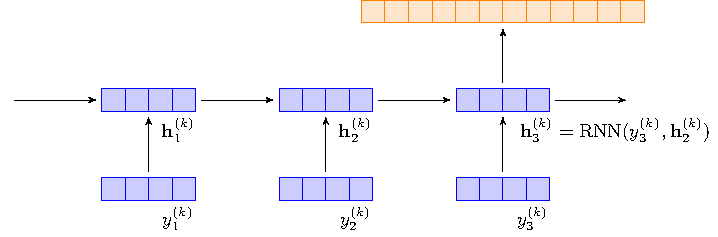
\includegraphics[scale=0.7]{rnntikzpicz/predrnnlm}
\end{center}


%\item Score of $t$'th word following history $y_{1:t-1}^{(k)}$:
\begin{align*}
s(w, \hat{y}_{1:t-1}^{(k)}) &= \only<1>{\log p(\hat{y}^{(k)}_{1:t-1}| x) + \log \softmax(\mathbf{W}_{out} \, \mathbf{h}_{t-1}^{(k)} + \mathbf{b}_{out})}\only<2->{\tst{\log p(\hat{y}^{(k)}_{1:t-1}| x) + \log \softmax(\mathbf{W}_{out} \, \mathbf{h}_{t-1}^{(k)} + \mathbf{b}_{out})}} \\
\only<2->{&= \mathbf{W}_{out} \, \mathbf{h}_{t-1}^{(k)} + \mathbf{b}_{out}}
\end{align*}

\air
\air
\only<3>{
\begin{itemize}
\item Can set $s(w, \hat{y}_{1:t-1}^{(k)}) \niceq {-}\infty$ if $(w, \hat{y}_{1:t-1}^{(k)})$ violates a hard constraint
\end{itemize}
}
\end{frame}

\begin{frame}[fragile]
  
    \begin{center}
      \textbf{Beam Search Optimization}
    \air
    \air
    \air
    \air

  \begin{tikzpicture}[transform canvas = {scale=0.8}]
  \tikzstyle{beam}=[draw, minimum height=0.6cm, anchor=base, text height=5, text depth=0, minimum width=1.5cm,thin, rounded corners, line width=0.03cm]
  \tikzstyle{mat}=[draw=white]
\tikzset{>=stealth',every on chain/.append style={join},
         every join/.style={->}}

     
       % \node[draw = white, yshift=1.8cm]{Time Step};
       %\node[draw = white, xshift=-7.5cm, yshift=0.5cm]{Beam:};
       \begin{scope}
         

   \matrix (G) [matrix of nodes, nodes={beam},inner sep=1mm,row sep=0.03cm, column sep=0.8cm ] {
    \node<1->[fill=yellow](G-1-1){\textcolor{blue}{a}}; & \node<2->[fill=yellow](G-1-2){red}; & \node<3->[fill=lightgray](G-1-3){\textcolor{blue}{dog}}; & \node<4->(G-1-4){smells}; & \node<8->[fill=lightgray](G-1-5){\textcolor{red}{home}};  & \node<9->(G-1-6){{today}}; \\
    \node<1->(G-2-1){the}; & \node<2->(G-2-2){dog}; & \node<3->[fill=yellow](G-2-3){dog}; & \node<4->(G-2-4){barks}; & \node<8->[fill=yellow](G-2-5){quickly}; & \node<9->(G-2-6){Friday}; \\
    \node<1->(G-3-1){red}; & \node<2->[fill=lightgray](G-3-2){\textcolor{blue}{blue}}; & \node<3->(G-3-3){cat}; &  \node<4->[fill=lightgray](G-3-4){\textcolor{blue}{barks}}; & \node<8->(G-3-5){straight}; & \node<9->[fill=lightgray](G-3-6){\textcolor{red}{now}}; \\
    & & & \node<4->[fill=yellow](G-4-4){runs}; & & \node<9->[fill=yellow](G-4-6){today}; \\
    };

    \only<2->{
      \draw[->] (G-1-1.east) -> (G-1-2.west); 
      \draw[->] (G-2-1.east) -> (G-2-2.west); 
      \draw[->] (G-1-1.east) -> (G-3-2.west); 
      \draw[double, line width=0.03cm] (G-3-1.south west) -- (G-3-2.south east);
    }
  
    \only<3->{
      \draw[->] (G-1-2.east) -> (G-2-3.west); 
      \draw[->] (G-3-2.east) -> (G-3-3.west); 
      \draw[->] (G-3-2.east) -> (G-1-3.west); 
      \draw[double, line width=0.03cm] (G-3-1.south west) -- (G-3-3.south east);
    }
    
 \only<4->{
    \draw[->] (G-2-3.east) -> (G-4-4.west); 
    \draw[->] (G-1-3.east) -> (G-3-4.west); 
    \draw[->] (G-2-3.east) -> (G-2-4.west); 
    \draw[->] (G-1-3.east) -> (G-1-4.west); 
    \draw[double, line width=0.03cm] (G-3-1.south west) -- (G-3-4.south east);
}

 \only<9->{
    \draw[->] (G-1-5.east) -> (G-1-6.west); 
    \draw[->] (G-1-5.east) -> (G-3-6.west); 
    \draw[->] (G-2-5.east) -> (G-2-6.west); 
    \draw[->] (G-2-5.east) -> (G-4-6.west); 
    \draw[double, line width=0.03cm] (G-3-1.south west) -- (G-3-6.south east);
}

    % \draw[->] (G-3-2.east) -> (G-3-3.west); 
    % \draw[->] (G-3-2.east) -> (G-1-3.west); 

 \only<8->{
    \draw[->, dashed] (G-4-4.east) -> (G-1-5.west); 
    \draw[->, dashed] (G-4-4.east) -> (G-2-5.west); 
    \draw[->, dashed] (G-4-4.east) -> (G-3-5.west); 
    \draw[double, line width=0.03cm] (G-3-1.south west) -- (G-3-5.south east);
}

       \end{scope}
\end{tikzpicture}
  \end{center}  

  \air 
  \air 
  \air 
  \only<-4>{
 \begin{align*}
 \mathcal{L}&(\theta) = \sum_{t} \Delta(\hat{y}_{1:t}^{(K)}) \left[1  - s(y_t, y_{1:t-1}) + s(\hat{y}_t^{(K)}, \hat{y}_{1:t-1}^{(K)}) \right] 
\end{align*}}  
  \only<5->{
 \begin{align*}
 \mathcal{L}&(\theta) = \sum_{t} \Delta(\hat{y}_{1:t}^{(K)}) \left[1  - \colorbox{yellow}{\strut$s(y_t, y_{1:t-1})$} + \colorbox{lightgrey}{\strut$s(\hat{y}_t^{(K)}, \hat{y}_{1:t-1}^{(K)})$} \right] 
\end{align*}}

\only<-4>{
  \begin{itemize}
  \item Color \textcolor{yellow}{Gold}: target sequence $y$
  \air
  \item Color \textcolor{gray}{Gray}: violating sequence $\hat{y}^{(K)}$

\vspace*{0.7cm}
 \end{itemize}
}
% \only<5-7>{
% \begin{itemize}
%   \item<5-> Need to BPTT for both $y_{1:t}$ and $\hat{y}_{1:t}^{(K)}$, which is $O(T)$
%   \air
%   \item<6-> Worst case: violation at each $t$ gives $O(T^2)$ backward pass
%   \air
%   \item<7-> \textbf{Idea:} use LaSO~\citep{daume05learning} beam-update
%   \end{itemize}
% }
\only<5->{
\vspace*{0.70cm}
\textbf{LaSO}~\citep{daume05learning}:
\begin{itemize}
\item  If no margin violation at $t\,{-}\,1$, update beam as usual
\air
\item Otherwise, update beam with sequences prefixed by $y_{1:t-1}$
\end{itemize}
}
%\centerline{Loss}
%  \vspace{-0.5cm}

\end{frame}

%\begin{frame}
%\frametitle{Efficiency Concerns}
%
%\begin{align*}
% \mathcal{L}&(\theta) = \sum_{t} \Delta(\hat{y}_{1:t}^{(K)}) \left[1 - \colorbox{yellow}{\strut$f(y_t, y_{1:t-1}, \boldx)$} +  \colorbox{lightgrey}{\strut$f(\hat{y}_t^{(K)}, \hat{y}_{1:t-1}^{(K)}, \boldx)$} \right] 
%\end{align*}
%
%\begin{itemize}
%\item Get gradients for gold sequence \textit{and} $K$'th sequence on the beam
%\air
%\item $\frac{\partial \mcL}{\partial f(y_{1:t})}$ and $\frac{\partial \mcL}{\partial f(\hat{y}_{1:t}^{(K)})}$ each require BPTT, which is $O(T)$
%\air
%\item Worst case: margin violation at each $t$ gives $O(T^2)$ for full backward pass
%\end{itemize}
%
%\end{frame}
%
%\begin{frame}
%\frametitle{Getting an $O(T)$ Backward Pass}
%\textbf{Idea:} use LaSO~\citep{daume05learning} search-update:
%\air
%\begin{itemize}
%\item If no margin violation at $t-1$, set beam at time $t$ as usual
%\air
%\item Otherwise, set beam at $t$ to contain \textit{only} sequences with $y_{1:t-1}$ as a prefix
%\end{itemize}
%\end{frame}

\begin{frame}[fragile]
  \centerline{\textbf{Backpropagation over Structure}}
  \begin{center}
    
  \air 
  \air 
  \air 

  \begin{tikzpicture}[transform canvas = {scale=0.8}]
    \tikzstyle{beam}=[draw, minimum height=0.6cm, anchor=base, text height=5, text depth=0, minimum width=1.5cm,thin, rounded corners, line width=0.03cm]
    \tikzstyle{mat}=[draw=white]
    \tikzset{>=stealth',every on chain/.append style={join},
      every join/.style={->}}
    
     
       % \node[draw = white, yshift=1.8cm]{Time Step};
       %\node[draw = white, xshift=-7.5cm, yshift=0.5cm]{Beam:};
       \begin{scope}
         

   \matrix (G) [matrix of nodes, nodes={beam},inner sep=1mm,row sep=0.03cm, column sep=0.8cm ] {
     \node[fill=yellow](G-1-1){\textcolor{blue}{a}}; & \node[fill=yellow](G-1-2){red}; & \node[fill=lightgray](G-1-3){\textcolor{blue}{dog}}; & \node(G-1-4){smells}; & \node[fill=lightgray](G-1-5){\textcolor{red}{home}};  & \node(G-1-6){{today}}; \\
     \node(G-2-1){the}; & \node(G-2-2){dog}; & \node[fill=yellow](G-2-3){dog}; & \node(G-2-4){barks}; & \node[fill=yellow](G-2-5){quickly}; & \node(G-2-6){Friday}; \\
     \node(G-3-1){red}; & \node[fill=lightgray](G-3-2){\textcolor{blue}{blue}}; & \node(G-3-3){cat}; &  \node[fill=lightgray](G-3-4){\textcolor{blue}{barks}}; & \node(G-3-5){straight}; & \node[fill=lightgray](G-3-6){\textcolor{red}{now}}; \\
     & & & \node[fill=yellow](G-4-4){runs}; & & \node[fill=yellow](G-4-6){today}; \\
    };


    \draw[->] (G-1-1.east) -> (G-1-2.west); 
    \draw[->] (G-2-1.east) -> (G-2-2.west); 
    \draw[->] (G-1-1.east) -> (G-3-2.west); 
    \draw[double, line width=0.03cm] (G-3-1.south west) -- (G-3-2.south east);


    \draw[->] (G-1-2.east) -> (G-2-3.west); 
    \draw[->] (G-3-2.east) -> (G-3-3.west); 
    \draw[->] (G-3-2.east) -> (G-1-3.west); 
    \draw[double, line width=0.03cm] (G-3-1.south west) -- (G-3-3.south east);

    \draw[->] (G-2-3.east) -> (G-4-4.west); 
    \draw[->] (G-1-3.east) -> (G-3-4.west); 
    \draw[->] (G-2-3.east) -> (G-2-4.west); 
    \draw[->] (G-1-3.east) -> (G-1-4.west); 
    \draw[double, line width=0.03cm] (G-3-1.south west) -- (G-3-4.south east);

    \draw[->] (G-1-5.east) -> (G-1-6.west); 
    \draw[->] (G-1-5.east) -> (G-3-6.west); 
    \draw[->] (G-2-5.east) -> (G-2-6.west); 
    \draw[->] (G-2-5.east) -> (G-4-6.west); 
    \draw[double, line width=0.03cm] (G-3-1.south west) -- (G-3-6.south east);


    % \draw[->] (G-3-2.east) -> (G-3-3.west); 
    % \draw[->] (G-3-2.east) -> (G-1-3.west); 


    \draw[->, dashed] (G-4-4.east) -> (G-1-5.west); 
    \draw[->, dashed] (G-4-4.east) -> (G-2-5.west); 
    \draw[->, dashed] (G-4-4.east) -> (G-3-5.west); 
    \draw[double, line width=0.03cm] (G-3-1.south west) -- (G-3-5.south east);


       \end{scope}

       \begin{scope}[yshift=-2.8cm]

      \matrix (G) [matrix of nodes,nodes={beam}, inner sep=1mm,row sep=0.06cm,column sep=0.8cm ] {
        \node[fill=yellow](G-1-1){a}; & \node[fill=yellow](G-1-2){red}; & \node[fill=yellow](G-1-3){dog}; & \node[fill=yellow](G-1-4){runs}; & \node[fill=yellow](G-1-5){quickly}; & \node[fill=yellow](G-1-6){today}; \\
         & \node[fill=lightgray](G-2-2){\textcolor{blue}{blue}}; & \node[fill=lightgray](G-2-3){\textcolor{blue}{dog}}; & \node[fill=lightgray](G-2-4){\textcolor{blue}{barks}}; & \node[fill=lightgray](G-2-5){\textcolor{red}{home}}; & \node[fill=lightgray](G-2-6){\textcolor{red}{now}}; \\
      };
    \draw[->] (G-1-1.east) -> (G-1-2.west); 
    \draw[->] (G-1-2.east) -> (G-1-3.west); 
    \draw[->] (G-1-3.east) -> (G-1-4.west); 
    \draw[->] (G-1-4.east) -> (G-1-5.west); 
    \draw[->] (G-1-5.east) -> (G-1-6.west); 

    \draw[->] (G-1-1.east) -> (G-2-2.west); 
    \draw[->] (G-2-2.east) -> (G-2-3.west); 
    \draw[->] (G-2-3.east) -> (G-2-4.west); 
    \draw[->] (G-1-4.east) -> (G-2-5.west); 
    \draw[->] (G-2-5.east) -> (G-2-6.west); 
      
    \end{scope}
  \end{tikzpicture}  
  \end{center}
  \vspace{2cm}
  \vspace{1cm}
  
  % \begin{itemize}
  % \item Margin gradients are sparse, only violating sequences get updates.
  % \item Backprop only requires 2x time as standard methods. 
  % \end{itemize}
\end{frame}

%\begin{frame}
%\frametitle{LaSO-style Search (with Constraints)}
%
%\begin{enumerate}
%\item[(1)] Initialize (empty) beam of hypotheses $\hat{y}_{1:0}^{(1:K)}$
%\air
%\item[(2)] For $t \niceq 1 \ldots T$:
%   \begin{enumerate}
%   \item[(a)] Compute for all $k$ and all possible output words $w$:
%     \begin{align*}
%     \hspace*{-4cm} s(\hat{y}_t \niceq w, \hat{y}_{1:t-1}^{(k)}) \gets f(\hat{y}_t^{(k)} \niceq w, \hat{y}_{1:t-1}^{(k)})
%     \end{align*}
%   \item[(b)] Reset beam:
%\begin{align*}
%          \hat{y}_{1:t}^{(1:K)} \gets \topK_{s} \begin{cases}  \lbrace \mcV \times {y}_{1:t-1} \mid (w, y_{1:t-1}) \text{ valid } \rbrace &\mbox{violation at $t$} \\
%     \lbrace \mcV \times \hat{y}_{1:t-1}^{(1:K)} \mid (w, \hat{y}_{1:t-1}^{(k)}) \text{ valid } \rbrace &\mbox{otherwise} \end{cases}
%\end{align*} 
%\end{enumerate}
%\end{enumerate}
%\end{frame}

%\begin{frame}
%  \centerline{\structure{Related Work:} }
%  \air 
%  
%  % \pause
%
%  % Opinion: 
%  % \begin{itemize}
%  % \item 
%  %   DAD methods only address exposure bias, 
%  % \item RL is too strong a hammer .
%  % \end{itemize}
%
%  % \begin{itemize}
%  % \item 
%  % \end{itemize}
%\end{frame}

 \begin{frame}
   \begin{center}
     \textbf{Recent Related Word}
   \end{center}
   \begin{itemize}
   \item Approaches to Exposure Bias, Label Bias:
  \begin{itemize}
  \item Data as Demonstrator, Scheduled Sampling \citep{Venkatraman,bengio15scheduled}
  \item Globally Normalized Transition-Based Networks \citep{Andor2016}
  \end{itemize}
  \air
  \item RL-based approaches
  \begin{itemize}
  \item MIXER \citep{ranzato16sequence}
  \item Actor-Critic \citep{Bahdanau2016}
  \end{itemize}
  \air
  \item Training with beam-search attempts to offer similar benefits
  \begin{itemize}
  \item Uses fact that we typically have gold prefixes in supervised text-generation to avoid RL
\end{itemize}   
\end{itemize}

%\begin{itemize}
%   \item Initial results are quite promising (but not yet SoTA)
%     \air
%   \item Results suggest RL may be unnecessary for these types of supervised tasks
%   \air
%   \item After all, in supervised text-generation we have gold prefixes!
%   \end{itemize}
 \end{frame}


\begin{frame}

  Experiments run on three Seq2Seq baseline tasks:

  \begin{itemize}
  \item Word Ordering, Dependency Parsing, Machine Translation
  \end{itemize}
  
\air
\air

\begin{itemize}
\item Uses LSTM encoders and decoders, attention, input feeding
%\item The beam-search variant (BSO) is identical, but without the output softmax
\item All models trained with Adagrad~\citep{duchi2011adaptive}
\item Pre-trained with NLL; $K$ increased gradually
\item ``BSO'' uses unconstrained search; ``ConBSO'' uses constraints
\end{itemize} 
 
\end{frame}


\begin{frame}
  % \centerline{Results}
  \vspace{-0.2cm}
  \begin{table}
  \centering
    \small
  \begin{tabular}{lccc}
    \toprule
    & $K_e$ = 1 & $K_e$ = 5 & $K_e$ = 10 \\ 
    \midrule
     & \multicolumn{3}{c}{Word Ordering (BLEU) } \\ 
    \midrule
    seq2seq & 25.2 & 29.8 & 31.0 \\
    BSO     & 28.0 & 33.2 & 34.3 \\
    ConBSO & \textbf{28.6} & \textbf{34.3} & \textbf{34.5} \\
    \midrule
%   \end{tabular}
%   \label{tab:wo}
% \end{table}


% \begin{table}
%   \centering
%   \hspace*{-0.3cm}\begin{tabular}{lccc}
%     \toprule
    & \multicolumn{3}{c}{Dependency Parsing (UAS/LAS)\footnote{Note \citet{Andor2016} have SOA, with 94.41/92.55.} } \\ 
    % \midrule
    seq2seq & \textbf{87.33/82.26} & 88.53/84.16 & 88.66/84.33\\
    BSO & 86.91/82.11 & 91.00/\textbf{87.18} & 91.17/\textbf{87.41} \\
    ConBSO & 85.11/79.32 & \textbf{91.25}/86.92 & \textbf{91.57}/87.26 \\
    % \midrule
    % Andor & 93.17/91.18 & - & - \\ 
    % \bottomrule

    \midrule
    & \multicolumn{3}{c}{Machine Translation (BLEU) } \\ 
    % &  $K_e$ = 1 & $K_e$ = 5 & $K_e$ = 10 \\ 
    % \midrule
    seq2seq & 22.53 & 24.03 & 23.87 \\
    BSO, SB-$\Delta$, $K_t$=6 & \textbf{23.83} & \textbf{26.36} & \textbf{25.48} \\
    % \midrule
    XENT & 17.74 & 20.10 & 20.28 \\
    DAD & 20.12 & 22.25 & 22.40 \\ 
    MIXER & 20.73 & 21.81 & 21.83 \\    
    \bottomrule
  \end{tabular}
  \label{tab:mtfinal}
\end{table}

\end{frame}

% \begin{frame}
%   \centerline{\structure{Discussion}}

%   \air

%   \begin{itemize}
%   \item Initial results are quite promising (but not yet SoTA)
%     \air
%   \item Results versus RL indicate that sampling and baselines may be 
%     overkill for this type of supervised task. 
%     \air
%   \item
%   \end{itemize}
% \end{frame}

\begin{frame}
  \centerline{\structure{This Talk}}
  \air 
  \air

  \begin{itemize}
  \item \textcolor{gray}{How can we \textbf{interpret} these learned hidden representations? \Cite{Strobelt2016}}
    \air 
  \item  \textcolor{gray}{ How should we \textbf{train} these style of models? \Cite{Wiseman2016a}}
    \air 
  \item How can we \textbf{shrink} these models for practical applications?

    \air 
    \begin{center}
      \alert{Sequence-Level Knowledge Distillation }

      \Cite{Kim2016a} 

      
\includegraphics[width=2cm]{yoon}
    \end{center}

  \end{itemize}
\end{frame}


% \begin{frame}
%   \centerline{\textbf{Seq2Seq In Practice}}
%   \air

%   \centerline{\alert{Downsides}}

%   \begin{itemize}
%   \item Models are really big (MT model is 4 layers each of 1000 units, GNTM is 8 layers)
%   \item Beam search can be quite slow
%   \end{itemize}
% \end{frame}


\begin{frame}
\center
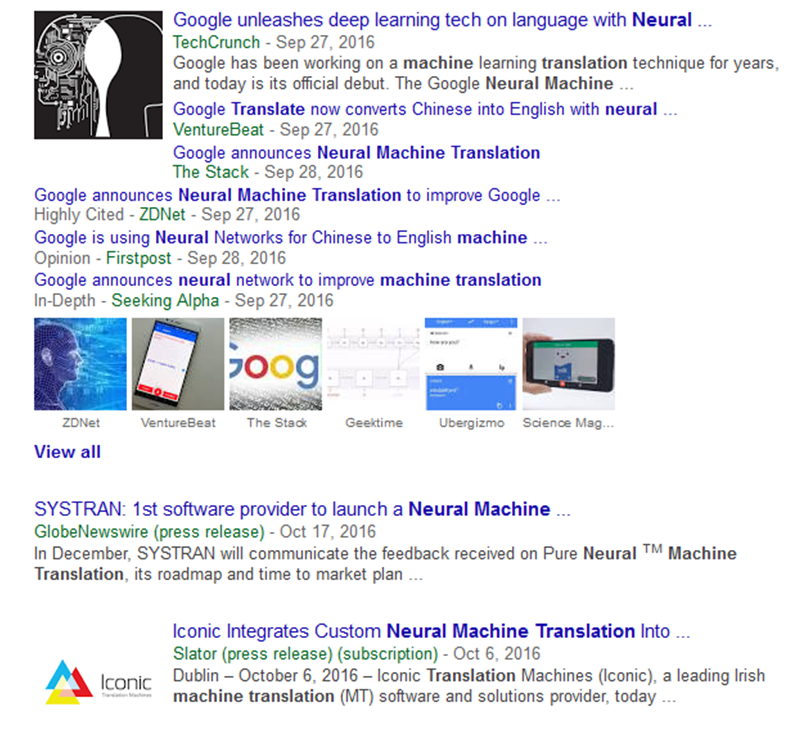
\includegraphics[scale=0.5]{nmt-news} \\
\end{frame}

\begin{frame}
\centerline{\structure{Neural Machine Translation}} \air \air
Excellent results on many language pairs, but need large models \air
\begin{itemize}
\item Original seq2seq paper \Cite{Sutskever2014}: 4-layers/1000 units
\item Deep Residual RNNs \Cite{Zhou2016} : 16-layers/512 units 
\item Google's NMT system \Cite{Wu2016}: 8-layers/1024 units 
\end{itemize}
\air 
\air 
\pause
Beam search + ensemble on top
\\ 
\air
$\implies$ Deployment is challenging! 
\end{frame}


\begin{frame}
  \centerline{\structure{Related Work: Compressing Deep Models}}
\air
\begin{itemize}
\item \textbf{Pruning}: Prune weights based on importance criterion 
\Cite{LeCun1990,Han2016,See2016}
\item \textbf{Knowledge Distillation}: Train a \textit{student} model to learn 
from a \textit{teacher} model \Cite{Bucila2006,Ba2014,Hinton2015,Kuncoro2016}. 
(Sometimes called ``dark knowledge'')
\end{itemize}
% \air
% \pause
%  Other methods: 
%  \begin{itemize}
%  \item low-rank matrix factorization of weight matrices \Cite{Denton2014}
%  \item weight binarization \Cite{Lin2016}
%  \item weight sharing \Cite{Chen2015}
%  \end{itemize}
\end{frame}

\begin{frame}
\centerline{\structure{Knowledge Distillation \Cite{Bucila2006,Hinton2015}}}
\air \air
\begin{itemize}
\item Train a \emph{larger teacher} model first to obtain teacher distribution $q(\cdot)$
\item Train a \emph{smaller student} model $p(\cdot)$ to mimic the teacher 
\end{itemize}
% \\ \\
% \air \air
% \end{frame}

% \begin{frame}
\pause
\air 
\alert{Word-Level Knowledge Distillation}
\air

Teacher distribution: $q(w_t \given y_{1:t-1})$ 
\begin{align*}
\mathcal{L}_{\text{NLL}} &=- \sum_t \sum_{k \in \mathcal{V}} {\color{red}{\mathbbm{1}\{y_t = k\}}} \log p(w_t = k \given  y_{1:t-1}; \theta) \\
\mathcal{L}_{\text{WORD-KD}} &=- \sum_t \sum_{k \in \mathcal{V}} {\color{blue}{q(w_t = k \given y_{1:t-1})}} \log p(w_t = k \given  y_{1:t-1}; \theta)
\end{align*}
\end{frame}

% \begin{frame}
% \centerline{\structure{No Knowledge Distillation}}
% \air 
% \center
% 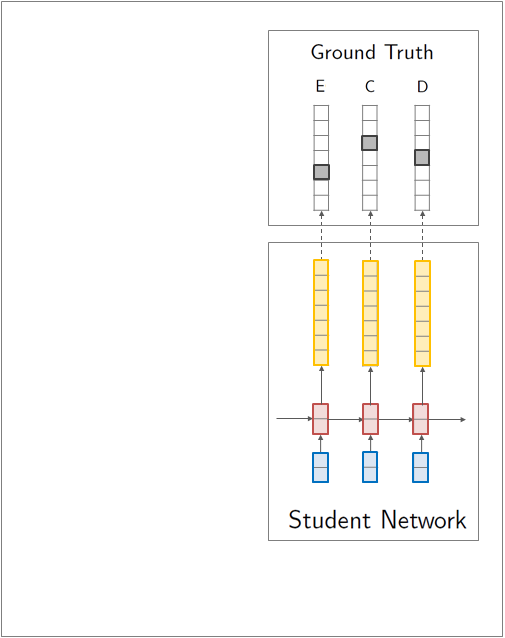
\includegraphics[width=6cm]{word-kd-0}
% \end{frame}

\begin{frame}
\centerline{\structure{Word-Level Knowledge Distillation}}
\air 
\begin{figure}
\center
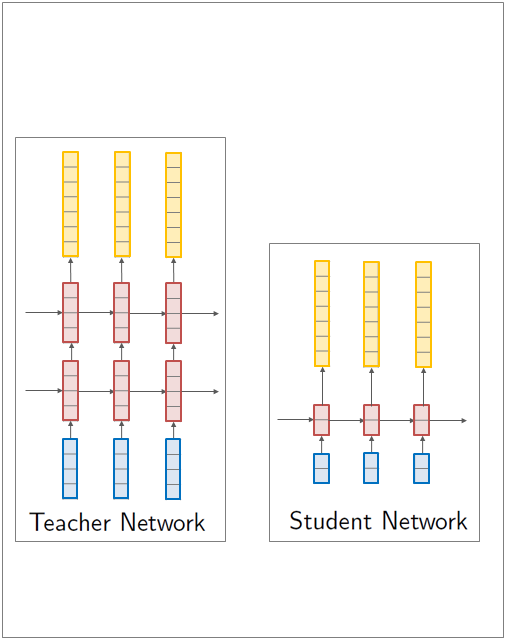
\includegraphics[width=6cm]{word-kd-1}
\end{figure}
\end{frame}

\begin{frame}
\centerline{\structure{Word-Level Knowledge Distillation}}
\air
\begin{figure} 
\center
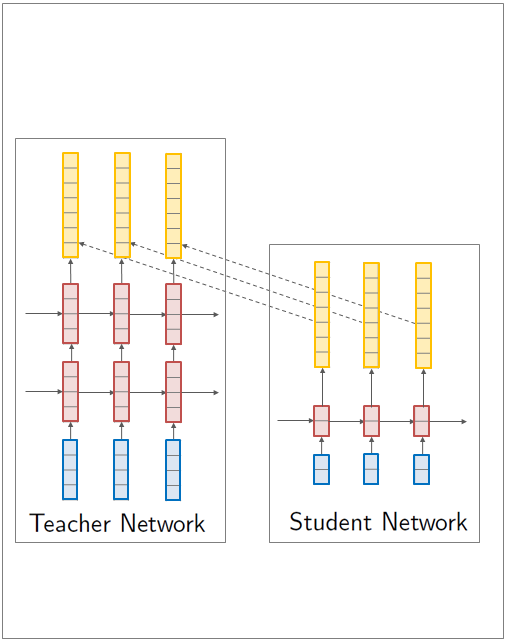
\includegraphics[width=6cm]{word-kd-2}
\end{figure}
\end{frame}

% \begin{frame}
% \centerline{\structure{Word-Level Knowledge Distillation}}
% \air 
% \center
% 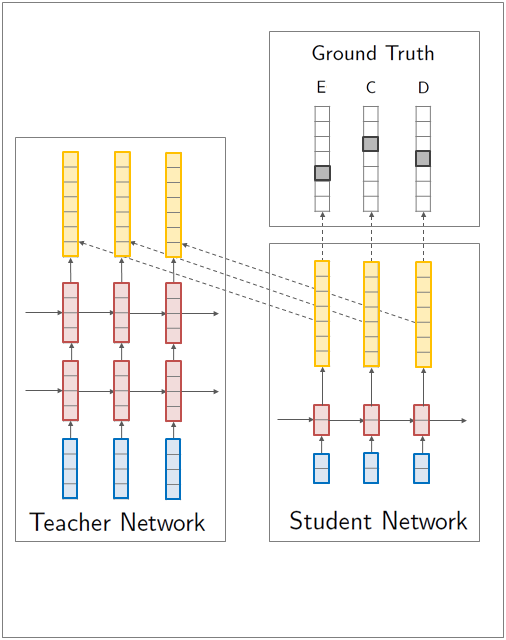
\includegraphics[width=5.5cm]{word-kd-3}
% $$\mathcal{L} = \alpha{\color{blue}{\mathcal{L}_{\text{WORD-KD}}}} + (1-\alpha){\color{red}{\mathcal{L}_{\text{NLL}}}}$$
% \end{frame}

% \begin{frame}
% \centerline{\structure{Baseline Model (No Knowledge Distillation)}}
% \air 

% \begin{columns}
% \begin{column}{6.5cm}
% Minimize NLL
% $$\mathcal{L}_{\text{NLL}} = -\sum_t \log p(y_t=\hat{y}_t \given \yvec_{1:t-1}, \xvec ; \theta)$$
% $y_t$ = $t$-th target token \\
% $\yvec_{1:t-1}$ = target sentence up to $t-1$ \\
% $\xvec$  = source sentence \\
% \air \air
% (conditioning on source $\xvec$ dropped from now on)
% \end{column}
% \begin{column}{5.5cm}
% 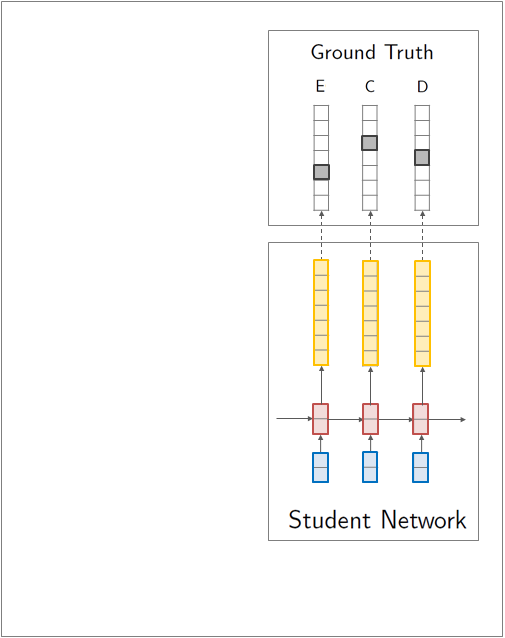
\includegraphics[width=5.5cm]{word-kd-0}
% \end{column}
% \end{columns}
% \end{frame}

% \begin{frame}
% \centerline{\structure{Word-Level Knowledge Distillation}}
% \air 
% \air

% \begin{columns}
% \begin{column}{6.5cm}
% Teacher network: $q(y_t \given \yvec_{1:t-1} ; \theta_T$)  \\
% \air
% \air
% Student network: $p(y_t \given \yvec_{1:t-1} ; \theta$)
% \end{column}
% \begin{column}{5.5cm}
% 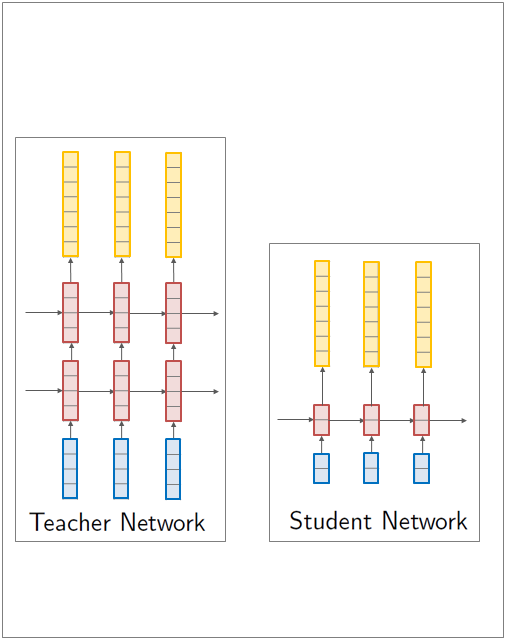
\includegraphics[width=5.5cm]{word-kd-1}
% \end{column}
% \end{columns}
% \end{frame}


% \begin{frame}

% \centerline{\structure{Word-Level Knowledge Distillation}}
% \air 
% \begin{columns}
% \begin{column}{6.5cm}

% Teacher network: $q(y_t | \yvec_{1:t-1}  ; \theta_T$)  
% \air 

% Minimize cross-entropy with teacher 
% \begin{align*}
% \mathcal{L}_{\text{WORD-KD}} = &  \\ -\sum_t \sum_{k \in \mathcal{V}} &q(y_t=k \given \yvec_{1: t-1} ; \theta_T)\times \\
% & \log p(y_t =k \given \yvec_{1: t-1} ; \theta)
% \end{align*}
% Sometimes $q$ and $p$ are annealed (i.e. $\tilde{q} \propto q^{\frac{1}{\tau}}$) to make it less peaky
% \end{column}

% \begin{column}{5.5cm}
% 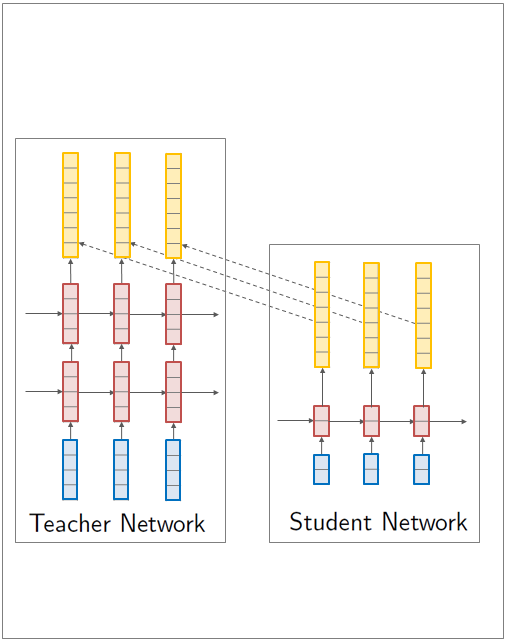
\includegraphics[width=5.5cm]{word-kd-2}
% \end{column}
% \end{columns}
% \end{frame}

% \begin{frame}
% \centerline{\structure{Word-Level Knowledge Distillation}}
% \air
% \begin{columns}
% \begin{column}{6.5cm}
% Add a term for NLL 
% $$\mathcal{L} = \alpha\mathcal{L}_{\text{WORD-KD}} + (1-\alpha)\mathcal{L}_{\text{NLL}}$$
% \air
% (we use $\alpha = 0.5$)
% \end{column}

% \begin{column}{5.5cm}
% 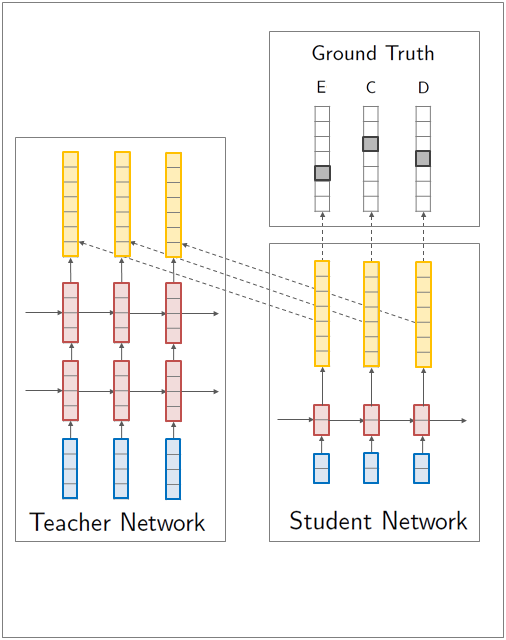
\includegraphics[width=5.5cm]{word-kd-3}
% \end{column}
% \end{columns}
% \end{frame}

\begin{frame}
\centerline{\structure{Word-Level Knowledge Distillation Results}}
\air
\air
\center English $\rightarrow$ German (WMT 2014)
\begin{table}
\centering
\small
\begin{tabular}{lc}
\toprule
Model &  BLEU   \\
\midrule
$4 \times 1000$  Teacher    &  $19.5$ \\
\midrule
$2 \times 500$ Baseline (No-KD)  $\,$   &  $17.6$   \\
$2 \times 500$ Student (Word-KD)  & $17.7$   \\
\midrule 
$2 \times 300$  Baseline (No-KD)  $\,$   &  $16.9$  \\
$2 \times 300$  Student (Word-KD)  &  $17.6$  \\
\bottomrule
\end{tabular}
\end{table}
\end{frame}

% \begin{frame}
% \centerline{\structure{This Work}}
% \air 
% \air
% Generalize single-class knowledge distillation to the sequence-level.
% \begin{itemize}
% \item \textbf{Sequence-Level Knowledge Distillation (Seq-KD)}: Train towards the teacher's sequence-level
% distribution.
% \item \textbf{Sequence-Level Interpolation (Seq-Inter)}: Train on a mixture of the teacher's distribution and the data.
% \end{itemize}
% \end{frame}

\begin{frame}
\centerline{\structure{This Work:  Sequence-Level Knowledge Distillation}}
\air 
\begin{align*}
\mathcal{L}_{\text{NLL}} &=- \sum_t \sum_{k \in \mathcal{V}} {\color{red}{\mathbbm{1}\{y_t = k\}}} \log p(w_t = k \given  y_{1:t-1}) \\
\mathcal{L}_{\text{WORD-KD}} &=- \sum_t \sum_{k \in \mathcal{V}} {\color{blue}{q(w_t = k \given y_{1:t-1})}} \log p(w_t = k \given  y_{1:t-1})
\end{align*}
\pause
Instead minimize cross-entropy, between $q$ and $p$ implied \emph{sequence}-distributions 
\begin{align*}
\mathcal{L}_\text{SEQ-KD} &=  -\sum_{w_{1:T} \in \mathcal{V}^T}{\color{blue}{q(w_{1:T} \given x)}}  \log p(w_{1:T} \given x  )
\end{align*}
\air
Sum over an exponentially-sized set $\mathcal{V}^T$. 
\end{frame}

\begin{frame}
\centerline{\structure{Sequence-Level Knowledge Distillation}}
\air 
\air
Approximate $q(w \given x )$ with mode
$$q(w_{1:T} \given x) \approx \mathbbm{1}\{\argmax_{w_{1:T}} q(w_{1:T} \given x )\}$$
\air
\pause
Approximate mode with  beam search 
$$ \hat{y} \approx  \argmax_{w_{1:T}} q(w_{1:T} \given x) $$
\pause
% Empirically, point estimate captures significant mass \\
% (Other approximations possible)

Simple model: train the student model on $\hat{y}$ with NLL
\end{frame}


\begin{frame}
\centerline{\structure{Sequence-Level Knowledge Distillation}}
\air 
\air
\begin{figure}
\center
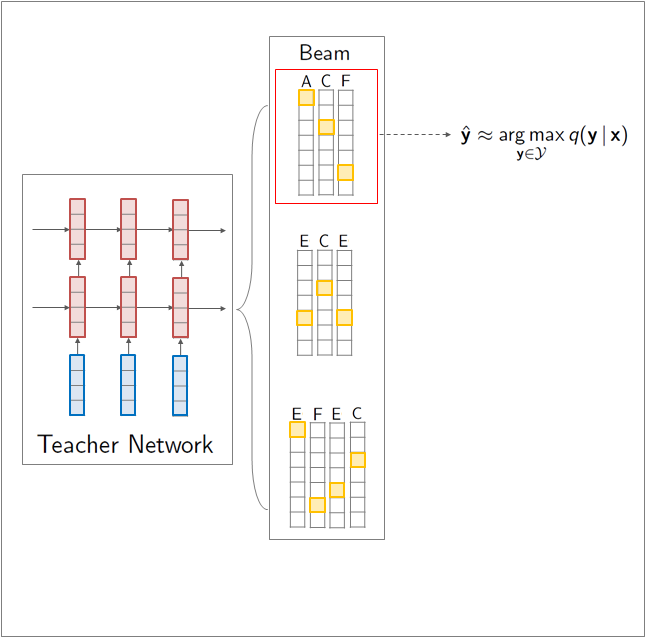
\includegraphics[width=7.5cm]{seq-kd-1}
\end{figure}
\end{frame}

\begin{frame}
\centerline{\structure{Sequence-Level Knowledge Distillation}}
\air
\air  
\begin{figure}
\center
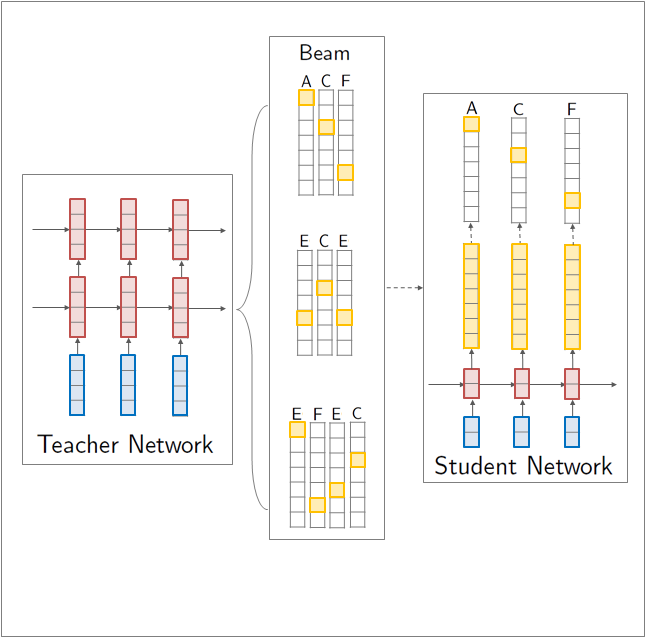
\includegraphics[width=7.5cm]{seq-kd-2}
\end{figure}
\end{frame}

% \begin{frame}
% \centerline{\structure{Sequence-Level Interpolation}}
% \air \air \air
% Word-level knowledge distillation
% $$\mathcal{L} = \alpha{\color{blue}{\mathcal{L}_{\text{WORD-KD}}}} + (1-\alpha)\color{red}{\mathcal{L}_{\text{NLL}}}$$
% Essentially training the student towards the mixture of teacher/data distributions. \\
% \air \air
% How can we incorporate ground truth data at the sequence-level?
% \end{frame}


% \begin{frame}
% \centerline{\structure{Sequence-Level Interpolation}}
% \air \air
% \begin{figure}
% \center
% 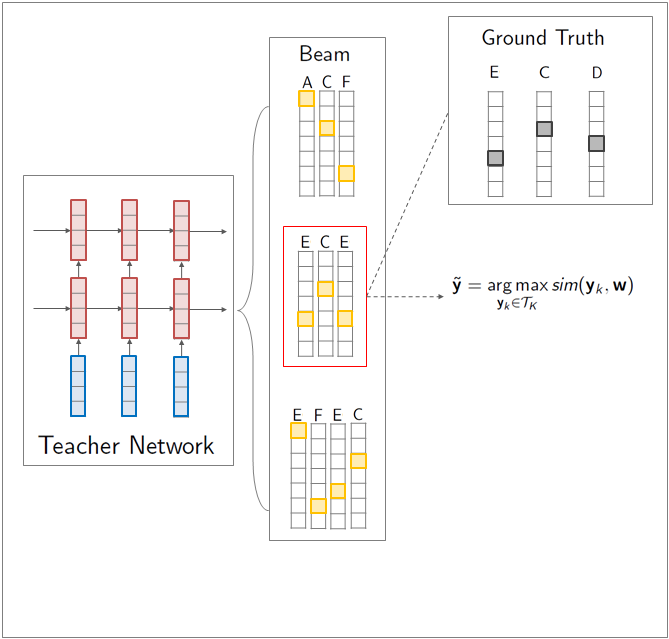
\includegraphics[width=7.5cm]{seq-inter-0}
% \end{figure}
% \end{frame}

% \begin{frame}
% \centerline{\structure{Sequence-Level Interpolation}}
% \air \air
% \begin{figure}
% \center
% 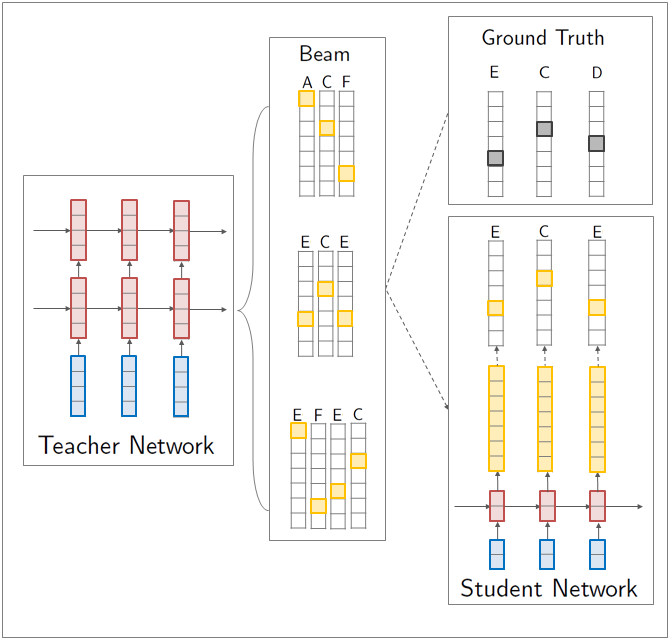
\includegraphics[width=7.5cm]{seq-inter-1}
% \end{figure}
% \end{frame}


\begin{frame}
\centerline{\structure{Experiments on English $\rightarrow$ German (WMT 2014)}}
\begin{itemize}
\item Word-KD: Word-level Knowledge Distillation
\item Seq-KD: Sequence-level Knowledge Distillation with beam size $K=5$
\item Seq-Inter: Sequence-level Interpolation with beam size $K=35$. Fine-tune
from pretrained Seq-KD (or baseline) model with smaller learning rate.
\end{itemize}
% Can mix configurations (e.g. train on Seq-KD data with word-level cross
% entropy against teacher)
\end{frame}

\begin{frame}
\centerline{\structure{Results: English $\rightarrow$ German (WMT 2014)}}
\air
\air
\begin{table}
\centering
\small
\begin{tabular}{lccccrr}
\toprule
Model &    BLEU$_{K=1}$   & $\Delta_{K=1}$ & BLEU$_{K=5}$ & $\Delta_{K=5}$ &  PPL & $p(\hat{\yvec})$ \\
\midrule
$4 \times 1000$ \\
Teacher    & $17.7$ &  $-$ & $19.5$&   $-$ &    $6.7$ &  $1.3\%$ \\
\only<5->{\hspace{1mm} Seq-Inter    & $19.6$ & $+1.9$&  $19.8$& $+0.3$&    $10.4$ & $8.2\%$}   \\
\midrule
$2 \times 500$ \\ 
Student  $\,$   & $14.7$ & $-$ & $17.6$&  $-$ &   $8.2$ & $0.9\%$  \\
\only<2->{\hspace{1mm} Word-KD  & $15.4$ & $+0.7$& $17.7$& $+0.1$&   $8.0$ & $1.0\%$}  \\
\only<3->{\hspace{1mm} Seq-KD   & $18.9$ & $+4.2$& $19.0$& $+1.4$&   $22.7$ & $16.9\%$} \\
\only<4->{\hspace{1mm} Seq-Inter  & $18.9$ & $+4.2$&$19.3$ & $+1.7$ &   $15.8$ & $7.6\%$}  \\
\bottomrule
\end{tabular}
\end{table}
\only<6>{\small Many more experiments (different language pairs, combining configurations, different sizes etc.) in paper}
\end{frame}

\begin{frame}
\centerline{\structure{An Application}}
\begin{center}

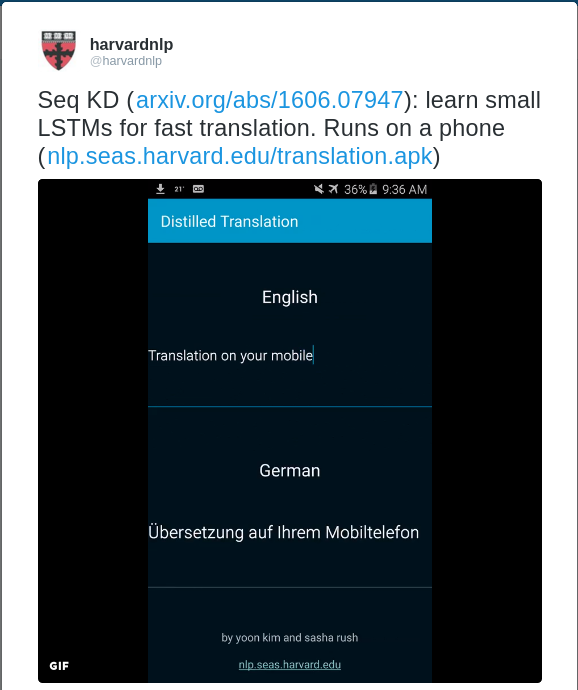
\includegraphics[width=5cm]{phonemt}
  \end{center}

  \href[pdfnewwindow=true]{https://harvardnlp.github.io/seq2seq-talk/transfast.gif}{[App]}
\end{frame}


\begin{frame}
\centerline{\structure{Decoding Speed}}
\center
\vspace{-5mm}
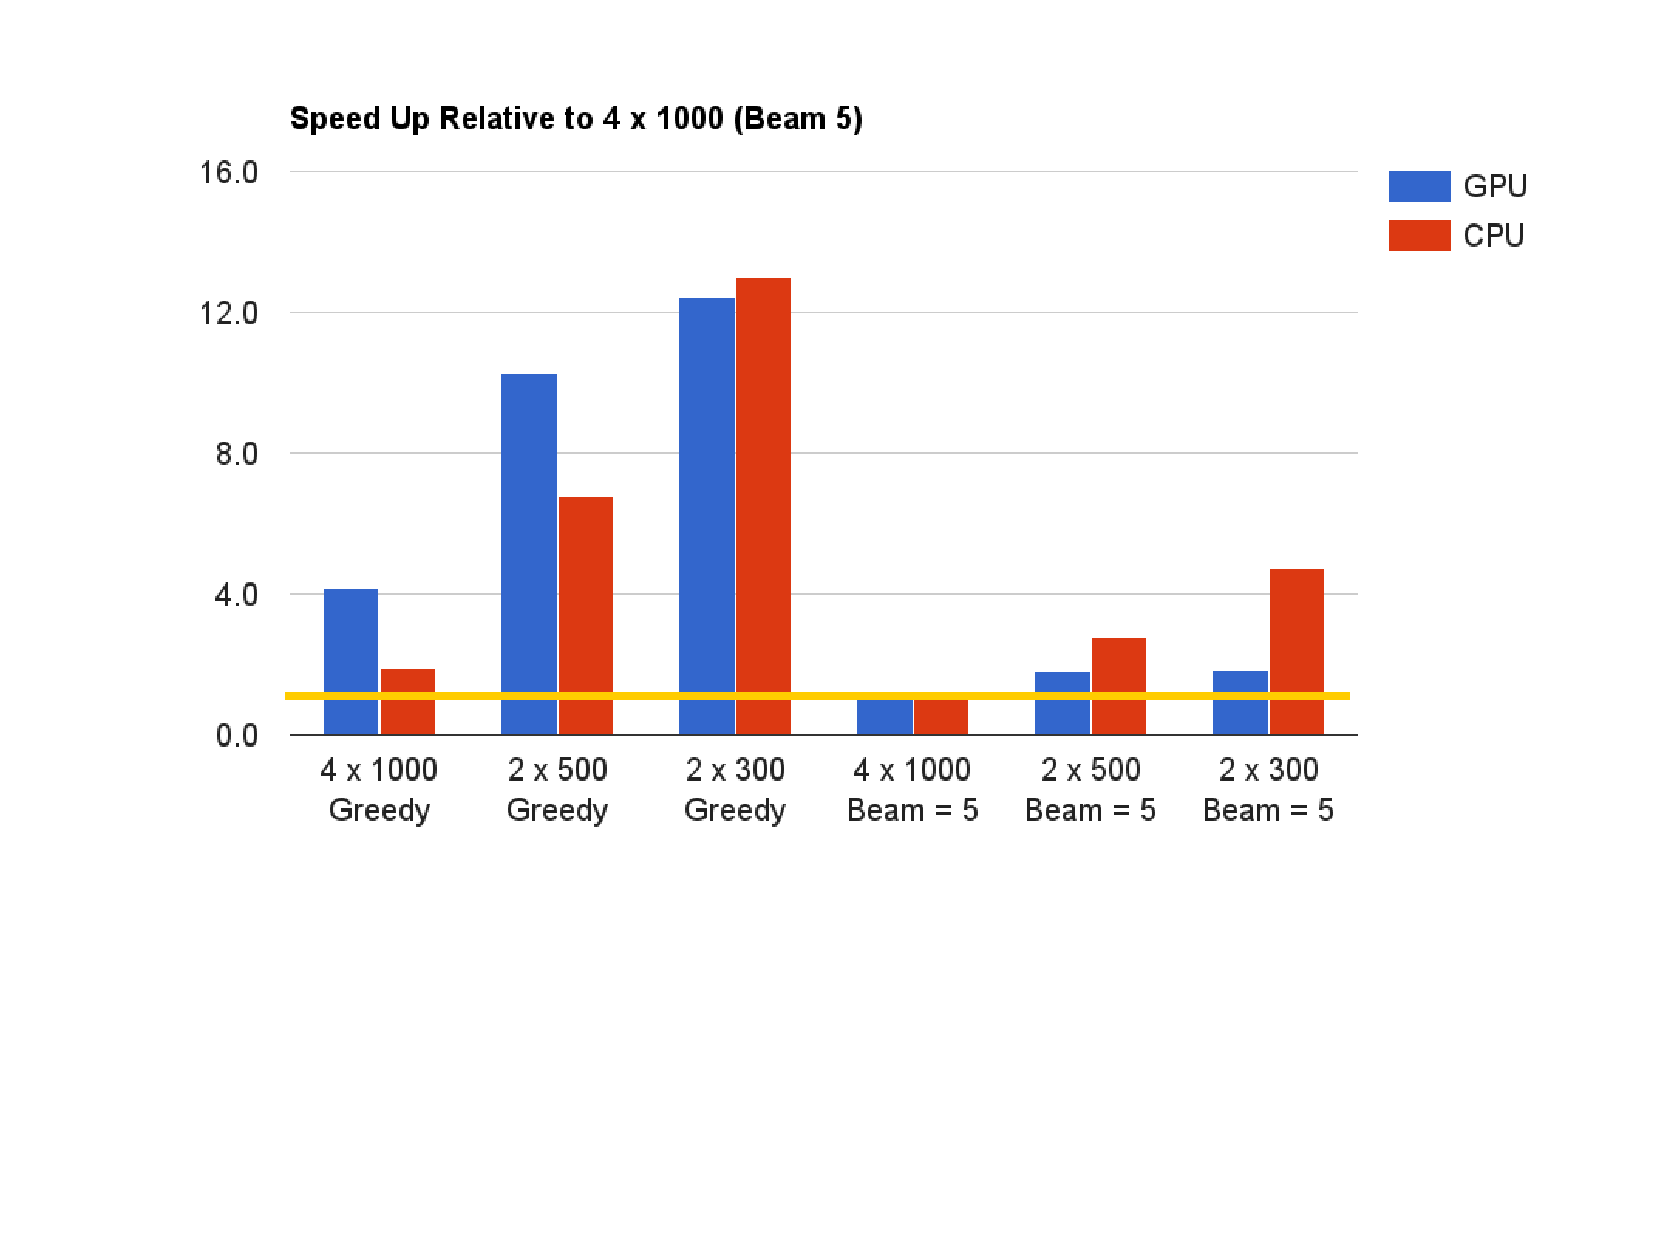
\includegraphics[scale=0.44]{dec-speed.pdf}
\end{frame}

\begin{frame}
  \begin{center} 
    \structure{Thank You}
  \end{center}
  \air 
  \begin{center}
    
\includegraphics[width=3cm]{harvardnlp}
  \end{center}
  % \structure{Focus:} Deep learning of the representation of language structure

  \begin{center}
    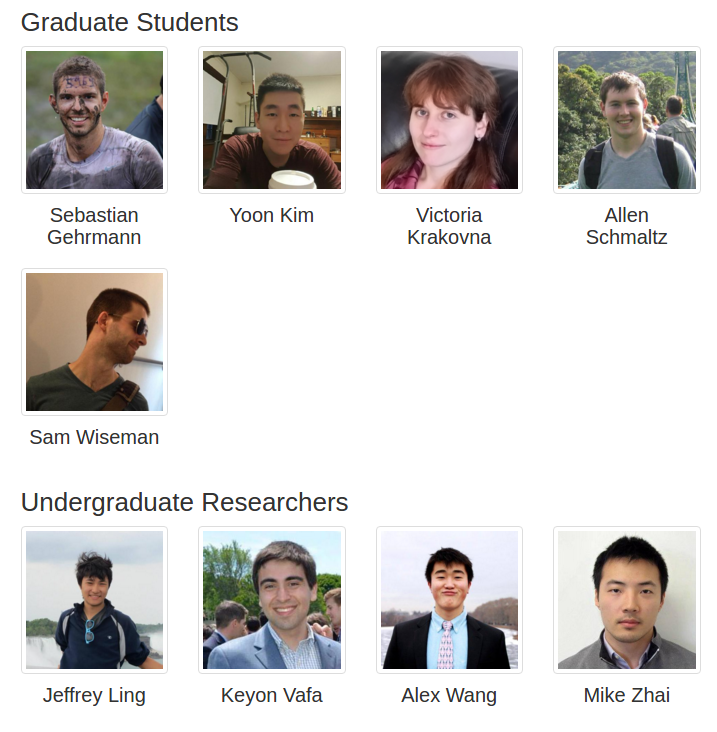
\includegraphics[width=6cm]{harvardnlpgroup}
  \end{center}
  
\end{frame}



\begin{frame}[t,allowframebreaks]
  \frametitle{References}
  \begin{small}
    \bibliography{full,career2,seq2seqapps,ourwork,master,masterseqk,beamtrain}
  \end{small}
 \end{frame}

\bibliographystyle{apalike}

\end{document}
